%-=-=-=-=-=-=-=-=-=-=-=-=-=-=-=-=-=-=-=-=-=-=-=-=
%        DOCUMENT
%-=-=-=-=-=-=-=-=-=-=-=-=-=-=-=-=-=-=-=-=-=-=-=-=
\documentclass[compress,newPxFont,sthlmFooter]{beamer}
\usetheme{sthlm} %Luebeck
%\usecolortheme{sthlmv42}

%-=-=-=-=-=-=-=-=-=-=-=-=-=-=-=-=-=-=-=-=-=-=-=-=
%        PACKAGES
%-=-=-=-=-=-=-=-=-=-=-=-=-=-=-=-=-=-=-=-=-=-=-=-=
% \usepackage[backend=biber, style=numeric]{biblatex}
\usepackage{biblatex}
% \bibliographystyle{apalike}
\newcommand{\skipcite}[1]{} 

\usepackage{colortbl}
\usepackage{graphbox}
\usepackage[absolute,overlay]{textpos}
\usepackage{hyperref}
\usepackage[utf8]{inputenc}
\usepackage[english,serbian]{babel}
\usepackage{xcolor}
\usepackage{chronology}
\renewcommand{\event}[3][e]{%
  \pgfmathsetlength\xstop{(#2-\theyearstart)*\unit}%
  \ifx #1e%
    \draw[fill=black,draw=none,opacity=0.5]%
      (\xstop, 0) circle (.2\unit)%
      node[opacity=1,rotate=45,right=.2\unit] {#3};%
  \else%
    \pgfmathsetlength\xstart{(#1-\theyearstart)*\unit}%
    \draw[fill=black,draw=none,opacity=0.5,rounded corners=.1\unit]%
      (\xstart,-.1\unit) rectangle%
      node[opacity=1,rotate=45,right=.2\unit] {#3} (\xstop,.1\unit);%
  \fi}%
  
\usepackage{amsmath}
\usepackage{amssymb,amsfonts,textcomp}
\usepackage{color}
\usepackage{placeins}
\usepackage{caption}
\usepackage{listings}
% \usepackage{droidmono}
\usepackage{subscript}

% \usecolortheme{default}
% \usefonttheme{professionalfonts}
% \usefonttheme[onlymath]{serif}

%-=-=-=-=-=-=-=-=-=-=-=-=-=-=-=-=-=-=-=-=-=-=-=-=
%        BEAMER OPTIONS
%-=-=-=-=-=-=-=-=-=-=-=-=-=-=-=-=-=-=-=-=-=-=-=-=
% \addbibresource{daetools.bib}

\setbeamertemplate{caption}{\insertcaption} 
\setbeamertemplate{caption label separator}{}

%\setbeameroption{show notes}
%\setbeamertemplate{note page}[plain]
%\setbeamertemplate{blocks}[rounded][shadow=true]
\definecolor{amethyst}{rgb}{0.6, 0.4, 0.8}
\definecolor{aogreen}{rgb}{0.0, 0.5, 0.0}
\definecolor{burgundy}{rgb}{0.5, 0.0, 0.13}
\definecolor{battleshipgrey}{rgb}{0.52, 0.52, 0.51}
\definecolor{light_red}{RGB}{255, 220, 220}
\definecolor{light_green}{RGB}{220, 255, 220}

\lstset{
    language=Python,
    basicstyle=\fontfamily{fdm}\scriptsize,
    keywordstyle=\color{blue},
    commentstyle=\color{aogreen},
    numberstyle=\color{battleshipgrey},
    stringstyle=\color{burgundy},
    identifierstyle=\color{black},
    frame=single,
    frameround=tttt,
    %numbers=left,
    keepspaces=true,
    showspaces=false,
    showtabs=false,
    showstringspaces=false,
    morekeywords={import, from, class, def, for, while, if, is, in, elif, else, not, and, or, print, break, 
                  continue, return, True, False, except, finally, import, lambda, pass, raise, try, None, __init__}
}

\lstset{
    language=C++,
    basicstyle=\fontfamily{fdm}\scriptsize,
    keywordstyle=\color{blue},
    commentstyle=\color{aogreen},
    numberstyle=\color{battleshipgrey},
    stringstyle=\color{burgundy},
    identifierstyle=\color{black},
    frame=single,
    frameround=tttt,
    %numbers=left,
    keepspaces=true,
    showspaces=false,
    showtabs=false,
    showstringspaces=false
}

\lstdefinestyle{gPROMS}{
    language=Python,
    basicstyle=\fontfamily{fdm}\scriptsize,
    keywordstyle=\color{blue},
    commentstyle=\color{aogreen},
    numberstyle=\color{battleshipgrey},
    stringstyle=\color{burgundy},
    identifierstyle=\color{black},
    frame=single,
    frameround=tttt,
    %numbers=left,
    keepspaces=true,
    showspaces=false,
    showtabs=false,
    showstringspaces=false,
    morekeywords={AS, EQUATION, PARAMETER, VARIABLE}
}

\lstdefinestyle{Modelica}{
    language=C++,
    basicstyle=\fontfamily{fdm}\scriptsize,
    keywordstyle=\color{blue},
    commentstyle=\color{aogreen},
    numberstyle=\color{battleshipgrey},
    stringstyle=\color{burgundy},
    identifierstyle=\color{black},
    frame=single,
    frameround=tttt,
    %numbers=left,
    keepspaces=true,
    showspaces=false,
    showtabs=false,
    showstringspaces=false,
    morekeywords={model, end, import, parameter, Real, equation, der}
}

% \setbeamertemplate{bibliography entry title}{}
% \setbeamertemplate{bibliography entry location}{}
% \setbeamertemplate{bibliography entry note}{}

%-=-=-=-=-=-=-=-=-=-=-=-=-=-=-=-=-=-=-=-=-=-=-=-=
%   PRESENTATION INFORMATION
%-=-=-=-=-=-=-=-=-=-=-=-=-=-=-=-=-=-=-=-=-=-=-=-=
\title{DAE Tools Software}
\subtitle{Introduction}
\author{D.D. Nikolić}
\institute
{
  DAE Tools Project, \url{http://www.daetools.com}
}
%\logo{
\includegraphics{../images/[d][a][e]_Tools_project.png}}
\date{1 June 2017} 

\hypersetup{
pdfauthor = {Dragan Nikolić: dnikolic@daetools.com},
pdfsubject = {Introduction to DAE Tools},
pdfkeywords = {Modelling, Simulation, Optimisation, Modelling languages, Model exchange, Domain
               specific languages, Equation-based, DAE, Code generation},
pdfmoddate= {D:\pdfdate},
pdfcreator = {Dragan Nikolić}
}

% \titlegraphic{
\includegraphics{../[d][a][e]_Tools_project.png}}

% \AtBeginSection[]
% {
%   \begin{frame}
%     \frametitle{Outline}
%     \tableofcontents[currentsection]
%   \end{frame}
% }
% 
\begin{document}

% \begin{frame}
% \titlepage
% \end{frame}
\maketitle

\begin{frame}{Outline}
\tableofcontents[sectionstyle=show, 
                 subsectionstyle=hide]
\end{frame} 

\section{General Information}

\begin{frame}{What is DAE Tools?} 
\alert{Modelling}, \alert{simulation}, \alert{optimisation} \& \alert{parameter estimation} software
\footnote{\tiny{Nikolić DD. (2016) \textit{DAE Tools: equation-based object-oriented modelling, simulation and optimisation software}.
          \href{https://doi.org/10.7717/peerj-cs.54}{PeerJ Computer Science 2:e54}}
         }

\begin{itemize}
  \item Areas of application:
    \begin{itemize}
      \item Initially: \alert{chemical process industry} (mass, heat and momentum transfers, chemical reactions, 
                                                          separation processes, thermodynamics, electro-chemistry)
      \item Nowadays: \alert{multi-domain}
    \end{itemize}
  \item \alert{Free/Open source software} (GNU GPL) 
\includegraphics[align=c,height=1.3em]{gnu_gpl3.png}
  \item \alert{Cross-platform} 
\includegraphics[align=c,height=1.3em]{linux.png} 
                               
\includegraphics[align=c,height=1.3em]{windows.png} 
                               
\includegraphics[align=c,height=1.3em]{macos.png}
  \item \alert{Multiple architectures} (32/64 bit x86, ARM, ...)
\end{itemize}
\end{frame}

\begin{frame}{What is DAE Tools? (cont'd)} 
  \begin{itemize}
    \item \textsc{DAE Tools} \alert{is not}:
        \begin{itemize}
            \item A modelling language (such as Modelica)
            \item An integrated software suite of data structures and routines for scientific applications (such as PETSc, Sundials, ...)
        \end{itemize}
    \item \textsc{DAE Tools} \alert{is}:
        \begin{itemize}
            \item An \alert{architectural design of interdependent software components}
                  providing an API for:
                \begin{itemize}
                    \item \alert{Model specification}
                    \item Activities on developed models (\alert{simulation}, \alert{optimisation}, ...)
                    \item \alert{Processing of the results}
                    \item \alert{Report generation}
                    \item \alert{Code generation} and \alert{model exchange}
                \end{itemize}
        \end{itemize}
    \item \textsc{DAE Tools} apply a \alert{hybrid approach} between \alert{modelling} and \alert{general purpose} programming languages,
          \alert{combining the strengths of both approaches} into a single one
  \end{itemize}
\end{frame}

\begin{frame}{What can be done with DAE Tools?} 
\begin{itemize}
  \item \alert{Simulation}
    \begin{itemize}
      \item Steady-State 
      \item Transient
    \end{itemize}
  \item \alert{Sensitivity analysis}
  \item \alert{Optimisation}
    \begin{itemize}
      \item Non-Linear Programming (NLP) problems
      \item Mixed Integer Non-Linear Programming (MINLP) problems
    \end{itemize}
  \item \alert{Parameter estimation}
  \item \alert{Code-generation}, \alert{model-exchange}, \alert{co-simulation} 
    \begin{itemize}
      \item Modelica, gPROMS
      \item Matlab MEX-functions, Simulink user-defined S-functions
      \item Functional Mockup Interface (FMI)
      \item C99 (for embedded systems)
      \item C++ MPI (for distributed computing) 
    \end{itemize}
\end{itemize}
\end{frame}

\begin{frame}{Types of systems that can be modelled}
  \alert{Initial value problems of implicit form}:
    \begin{itemize}
      \item Described by \alert{systems of linear, non-linear, and (partial-)differential} algebraic equations
      \item \alert{Continuous} with some elements of \alert{event-driven} systems 
            (discontinuous equations, state transition networks and discrete events) 
      \item \alert{Steady-state} or \alert{dynamic}
      \item With \alert{lumped} or \alert{distributed} parameters 
            (finite difference, finite volume and finite element methods)
      \item Only \alert{index-1} DAE systems at the moment
    \end{itemize}
\end{frame}

\section{Motivation}

\begin{frame}
\frametitle{Why modelling software?}
In general, two scenarios:
\begin{itemize}
  \item \alert{Development} of a \alert{new} product/process/...
    \begin{itemize}
        \item Reduce the time to market (TTM)
        \item Reduce the development costs (no physical prototypes)
        \item Maximise the performance, yield, productivity, purity, ...
        \item Minimise the capital and operating costs
        \item Explore the new design options in less time and no risks
    \end{itemize}

  \item \alert{Optimisation} of an \alert{existing} product/process/...
    \begin{itemize}
        \item Increase the performance, yield, productivity, purity, ...
        \item Reduce the operating costs, energy consumption, ...
        \item Debottleneck
    \end{itemize}
\end{itemize}
\end{frame}

\begin{frame}{Why \textsc{yet another} modelling software?}
Current approaches to mathematical modelling:
\begin{enumerate}
   \item Use of \alert{modelling languages} (domain-specific or multi-domain):
         \alert{Modelica}\skipcite{Fritzson-and-Engelson-1998}, 
         \alert{Ascend}\skipcite{Piela-etal-1991}, 
         \alert{gPROMS}\skipcite{Barton-and-Pantelides-1994}, 
         \alert{Dymola}\skipcite{Elmqvist-1978}, 
         \alert{APMonitor}\skipcite{APMonitor-2014}
   \item Use of \alert{general-purpose programming languages}:
      \begin{itemize}
          \item Lower level third-generation languages such as C, C++ and Fortran
                (\alert{PETSc}\skipcite{petsc}, 
                 \alert{SUNDIALS}\skipcite{Hindmarsh-etal-2005})
          \item Higher level fourth-generation languages such as \alert{Python} (NumPy, SciPy, Assimulo\skipcite{Assimulo-2015}), 
                                                                 \alert{Julia} etc.
          \item Multi-paradigm numerical languages 
                (\alert{Matlab}\skipcite{matlab}, 
                 \alert{Mathematica}\skipcite{mathematica}, 
                 \alert{Maple}\skipcite{maple}, 
                 \alert{Scilab}\skipcite{scilab}, and 
                 \alert{GNU Octave}\skipcite{octave})
      \end{itemize}
 \end{enumerate}
\end{frame}

\begin{frame}{Why \textsc{yet another} modelling software? (cont'd)}
  The advantages of the \alert{Hybrid} approach over the \alert{modelling} and \alert{general-purpose} programming languages:
    \begin{enumerate}
        \item Support for the \alert{runtime model generation}
        \item Support for the \alert{runtime simulation set-up}
        \item Support for \alert{complex schedules} (operating procedures)
        \item \alert{Interoperability} with the \alert{third-party software}
        \item Suitability for \alert{embedding} and use as a \alert{web application} or \alert{software as a service}
        \item \alert{Code-generation}, \alert{model exchange} and \alert{co-simulation} capabilities  
    \end{enumerate}
\end{frame}
% 
% \begin{frame}{Why \textsc{yet another} modelling software? (cont'd)}
%     The \alert{shovel metaphor} about cleaning the snow in the winter:
%     \begin{enumerate}
%        \item \alert{Pay someone} to do it 
%        \item \alert{Go shovel}
%     \end{enumerate}
% %     \begin{itemize}
% %         \item Cleaning the snow in the winter - \alert{pay someone} to do it or \alert{go shovel}?
% %         \begin{itemize}
% %             \item \alert{Paying someone is expensive} and \alert{easy}
% %             \item \alert{The shovel is cheap} but \alert{shoveling is hard}
% %             \item Shoveling is \alert{good for health} and \alert{you can shovel everyday}
% %         \end{itemize}
% %     \end{itemize}
%     
%     \scriptsize
%     {
%     \begin{table}
%     %\caption{Notate bene:}
%     \begin{tabularx}{\linewidth}{p{0.46\linewidth}X}
%         \toprule
%         \textbf{Paying for the service} & \textbf{Shovelling manually} \tabularnewline
%         \midrule
%         
%         Expensive but easy & The tool (shovel) is cheap but shoveling requires effort and training to do it 
%         \tabularnewline \midrule
%         
%         Depends on external man power & Can be done anytime
%         \tabularnewline \midrule
%         
%         Unavailable or very expensive (during Christmas, weekend, night)  & Can be done anytime 
%         \tabularnewline \midrule
%               
%         Delays from the call until execution & No delays can be done immediately
%         \tabularnewline \midrule
% 
%         Cannot be done urgently (what if a child is ill and has to go to the hospital) & Can be done anytime 
%         \tabularnewline
%         
%         \bottomrule
%     \end{tabularx}
%     \end{table}
%     }
% %                 Like with shoveling - they do not do it during weekends and bank holidays (or you can, but it costs a lot)
% \end{frame}
% 
% \begin{frame}{Why \textsc{yet another} modelling software? (cont'd)}
%   \begin{itemize}
%       \item \alert{Modelling} $\equiv$ \alert{cleaning the snow} in the winter
%         \begin{enumerate}
%             \item \alert{Pay someone} to do it 
%             \item \alert{Go shovel}
%         \end{enumerate}
% %       \item Modelling software does not do anything useful (it is just a tool, like a shovel)
% %       \item Model of a process/product is useful
% %       \item There are two ways to go:
% %         \begin{enumerate}
% %           \item Use one of the available commercial/proprietary software with a range of pre-built model libraries
% %                 You can pay for development of custom features
% %                 But once they build an extended library it will soon end up in the main version. 
% %                 You will essentially pay the development expenses for the modelling company
% %                 Also, the custom features cannot be built whenever they are needed - some time is required before thay come, make plans and develop it.
% %                 Like with shoveling - they do not do it during weekends and bank holidays (or you can, but it costs a lot)
% %           \item Use the free/open-source software to build the models
% %         \end{enumerate}
% %       \item Commercial products are like buy an expensive robot that does it autonomously 
% %             + it requires a mandatory yearly maintanance 
% %       \item \textsc{DAE Tools} is like buying a cheap shovel and do it manually
%   \end{itemize}
% \end{frame}

\begin{frame}{Additional \textsc{DAE Tools} features}
    \begin{itemize}
        \item Support for \alert{multiple platforms/architectures} 
        \item Support for the \alert{automatic differentiation} (ADOL-C)
        \item Support for the \alert{sensitivity analysis} through the auto-differentiation capabilities
        \item Support for the \alert{parallel} computation (OpenMP, GPGPU, MPI)
        \item Support for a large number of \alert{DAE}, \alert{LA} and \alert{NLP} solvers 
        \item Support for the generation of \alert{model reports} (XML + MathML, Latex)
        \item \alert{Export} of the \alert{simulation results} to various file formats (Matlab, Excel, json, xml, HDF5, Pandas, VTK)
    \end{itemize}
\end{frame}

\section{Programming Paradigms}

\begin{frame}{The \textsc{hybrid} approach}
  \begin{itemize}
    \item DAE Tools approach is a \alert{type of a hybrid approach}
    \item Combines strengths of \alert{modelling} and \alert{general purpose} programming languages:
        \begin{enumerate}
            \item \alert{Developed in C++} with the \alert{Python bindings}
            \item Provides \alert{API} (Application Programming Interface) that \alert{resembles a syntax of modelling languages}
                  as much as possible
            \item \alert{Takes advantage of the higher level languages} for:
                \begin{itemize}
                    \item Model specification, simulation setup and schedules
                    \item Access to the operating system 
                    \item Access to the standard/third-party libraries
                \end{itemize}
        \end{enumerate}
  \end{itemize}
\end{frame}

\begin{frame}[plain]{The \textsc{hybrid} approach (cont'd)}
    \begin{columns}[c]
      \begin{column}{0.7\paperwidth}
        {\small
         \begin{itemize}
            \item \textcolor{sthlmRed}{Modelica}/\textcolor{sthlmRed}{gPROMS} grammars vs. \textcolor{sthlmRed}{DAE Tools API} 
            \item A simple model: \newline
                    {\scriptsize
                        Cylindrical tank containing a liquid with an inlet and an outlet flow;  
                        the outlet flowrate depends on the liquid level in the tank
                    }
        \end{itemize}
        }
      \end{column}
      
      \begin{column}{0.3\paperwidth}
        \begin{center}
          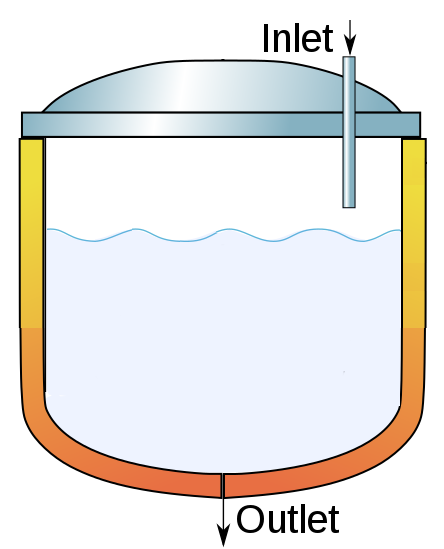
\includegraphics[align=c, width=0.17\paperwidth]{buffer_tank.png}
        \end{center}
      \end{column}
    \end{columns}

    \begin{columns}[b]
      \begin{column}{0.5\paperwidth}
        \begin{center}
           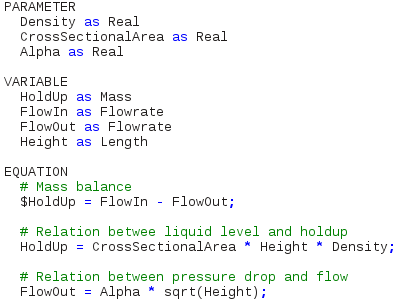
\includegraphics[align=c, width=0.35\paperwidth]{gproms_model.png} \par
           {\scriptsize \textcolor{sthlmRed}{gPROMS grammar}}
        \end{center}
      \end{column}
      \begin{column}{0.5\paperwidth}
        \begin{center}
           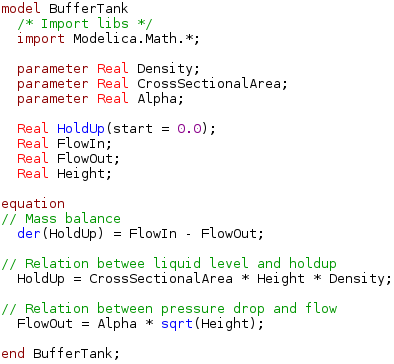
\includegraphics[align=c, width=0.35\paperwidth]{modelica_model.png} \par
           {\scriptsize \textcolor{sthlmRed}{Modelica grammar}} 
        \end{center}
      \end{column}
    \end{columns}
\end{frame}

\begin{frame}{The \textsc{hybrid} approach (cont'd)}
    \begin{center}
       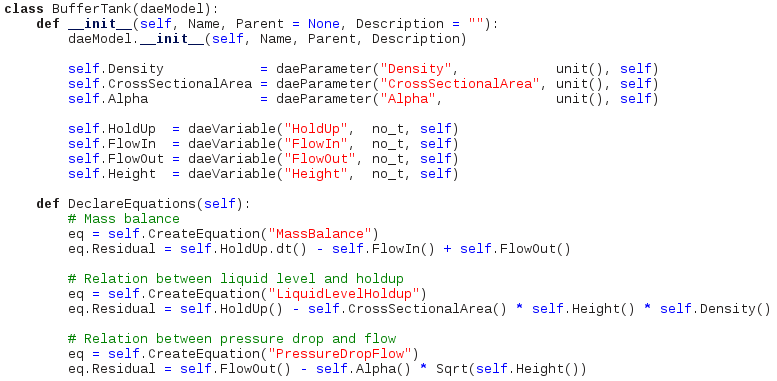
\includegraphics[align=c, width=0.70\paperwidth]{daetools_model.png} \par
       {\scriptsize \textcolor{sthlmRed}{DAE Tools API}}
    \end{center}
\end{frame}


\begin{frame}[plain]{The \textsc{hybrid} approach (cont'd)}
\tiny
{
\begin{table}
  \begin{tabularx}{\linewidth}{p{0.46\linewidth}X}
    \toprule
    \textcolor{sthlmRed}{\textbf{Modelling language approach}} & \textcolor{sthlmRed}{\textbf{DAE Tools approach}} \tabularnewline
    \midrule
    
    \cellcolor{light_green}Solutions expressed in the idiom and at the level of abstraction of the problem domain
      &
    \cellcolor{light_red}Must be emulated in the API or in some other way 
    \tabularnewline \midrule
    
    \cellcolor{light_green}Clean and concise way of building models
      &
    \cellcolor{light_red}Verbose and less elegant
    \tabularnewline \midrule
    
    \cellcolor{light_green}Could be and often are simulator independent
      &
    \cellcolor{light_red}Simulator dependent (but with code-generation) 
    \tabularnewline \midrule
    
    \cellcolor{light_red}Cost of designing, implementing, and maintaining a language and 
    a compiler/lexical parser/interpreter, error handling and grammar ambiguities
      &
    \cellcolor{light_green}A compiler/lexical parser/interpreter is an integral part of C++/Python with a
    robust error handling, universal grammar and massively tested 
    \tabularnewline \midrule
    
    \cellcolor{light_red}Cost of learning a new language vs. its limited applicability (yet another language grammar)
      &
    \cellcolor{light_green}No learning of a new language required
    \tabularnewline \midrule
    
    \cellcolor{light_red}Difficult to integrate with other components
      &
    \cellcolor{light_green}Calling external libraries is a built-in feature 
    \tabularnewline \midrule
    
    \cellcolor{light_red}Models usually cannot be created/modified in the runtime (or at least not easily)
      &
    \cellcolor{light_green}Models can be created/modified in the runtime 
    \tabularnewline \midrule
    
    \cellcolor{light_red}Setting up a simulation embedded in the language; difficult to obtain initial values from other software
      &
    \cellcolor{light_green}Setting up a simulation done programmaticaly and the initial values can be obtained from other software
    \tabularnewline \midrule
    
    \cellcolor{light_red}Schedules limited to the options allowed by the langueage grammar
      &
    \cellcolor{light_green}Schedules completely flexible (within the limits of a programming language itself)
    \tabularnewline
    
    \bottomrule
  \end{tabularx}
\end{table}
}
\end{frame}

\begin{frame}{The \textsc{object-oriented} approach}
\begin{itemize}
  \item Everything is an \alert{object} (variables, equations, models ...)
  \item All objects can be \alert{manipulated} in \alert{the runtime}
  \item \alert{All} C++/Python \alert{object-oriented concepts supported}
  \item Models, simulations, optimisations:
     \begin{itemize}
        \item \alert{Derived from} the corresponding \alert{base classes}
        \item \alert{Inherit} the \alert{common functionality} from the base classes
        \item Perform the \alert{functionality} in \alert{overloaded functions}
     \end{itemize}
  \item The \alert{hierarchical model decomposition} possible:
    \begin{itemize}
        \item Models can contain instances of other models
        \item Complex, re-usable model definitions can be created
        \item Models at different scales can be loosely coupled %(multi-scale modelling)
    \end{itemize}
\end{itemize}
\end{frame}

\begin{frame}{The \textsc{equation-oriented} (\textsc{acausal}) approach}
\begin{itemize}
  \item \alert{Equations given in an implicit form} (as a residual)
    \begin{center}
      $F(\dot {x}, x, y, p) = 0$
    \end{center}
  \item \alert{Input-Output causality} is \alert{not fixed}:
    \begin{itemize}
        \item Increased model re-use
        \item Support for \alert{different simulation scenarios} (based on a single model) by specifying different degrees of freedom
    \end{itemize}
  \item An example:
    \begin{itemize}
        \item The equation given in the following form:
            \begin{center}
                $x_1 + x_2 + x_3 = 0$
            \end{center}
        \item Can be used to determine either $x_1$, $x_2$ or $x_3$ depending on what combination of variables is known:
            \begin{center}
                $x_1 = -x_2 - x_3, \;$ \alert{or}  $\;$
                $x_2 = -x_1 - x_3, \;$ \alert{or}  $\;$
                $x_3 = -x_1 - x_2$
            \end{center}
    \end{itemize}
\end{itemize}
\end{frame}

\begin{frame}{Separation of \textsc{model definition} from its \textsc{applications}}
\begin{itemize}
  \item \alert{Model structure} specified in the \alert{model class}
  \item \alert{Runtime information} specified in the \alert{simulation class}
  \item \alert{Solvers/auxiliary objects} declared in the \alert{main program}
  \item \alert{Single model definition}, but \alert{one or more}:
  \begin{itemize}
    \item Different \alert{simulation scenarios}
    \item Different \alert{optimisation scenarios}
  \end{itemize}
\end{itemize}
\end{frame}

\section{Architecture}

\begin{frame}[plain]{The fundamental concepts/software interfaces}
\begin{columns}
    \begin{column}{0.28\paperwidth}
        \tiny{
        \begin{itemize}
            \item The main concepts:
                \begin{itemize}
                    \tiny{
                        \item \textcolor{sthlmRed}{daeModel\_t}
                        \item \textcolor{sthlmRed}{daeSimulation\_t}
                        \item \textcolor{sthlmRed}{daeOptimization\_t}
                        \item \textcolor{sthlmRed}{daeBlock\_t}
                        \item \textcolor{sthlmRed}{daeDAESolver\_t}
                        \item \textcolor{sthlmRed}{daeLASolver\_t}
                        \item \textcolor{sthlmRed}{daeDataReporter\_t}
                        \item \textcolor{sthlmRed}{daeBlock\_t}
                    }
                \end{itemize}
            \item In 6 packages:
                \begin{itemize}
                \tiny{
                        \item \alert{core}
                        \item \alert{activity}
                        \item \alert{datareporting}
                        \item \alert{solvers}
                        \item \alert{logging}
                        \item \alert{units}
                    }
                \end{itemize}
        \end{itemize}
        }
     \end{column}
     
     \begin{column}{0.72\paperwidth}
         \begin{center}
             \begin{figure}
               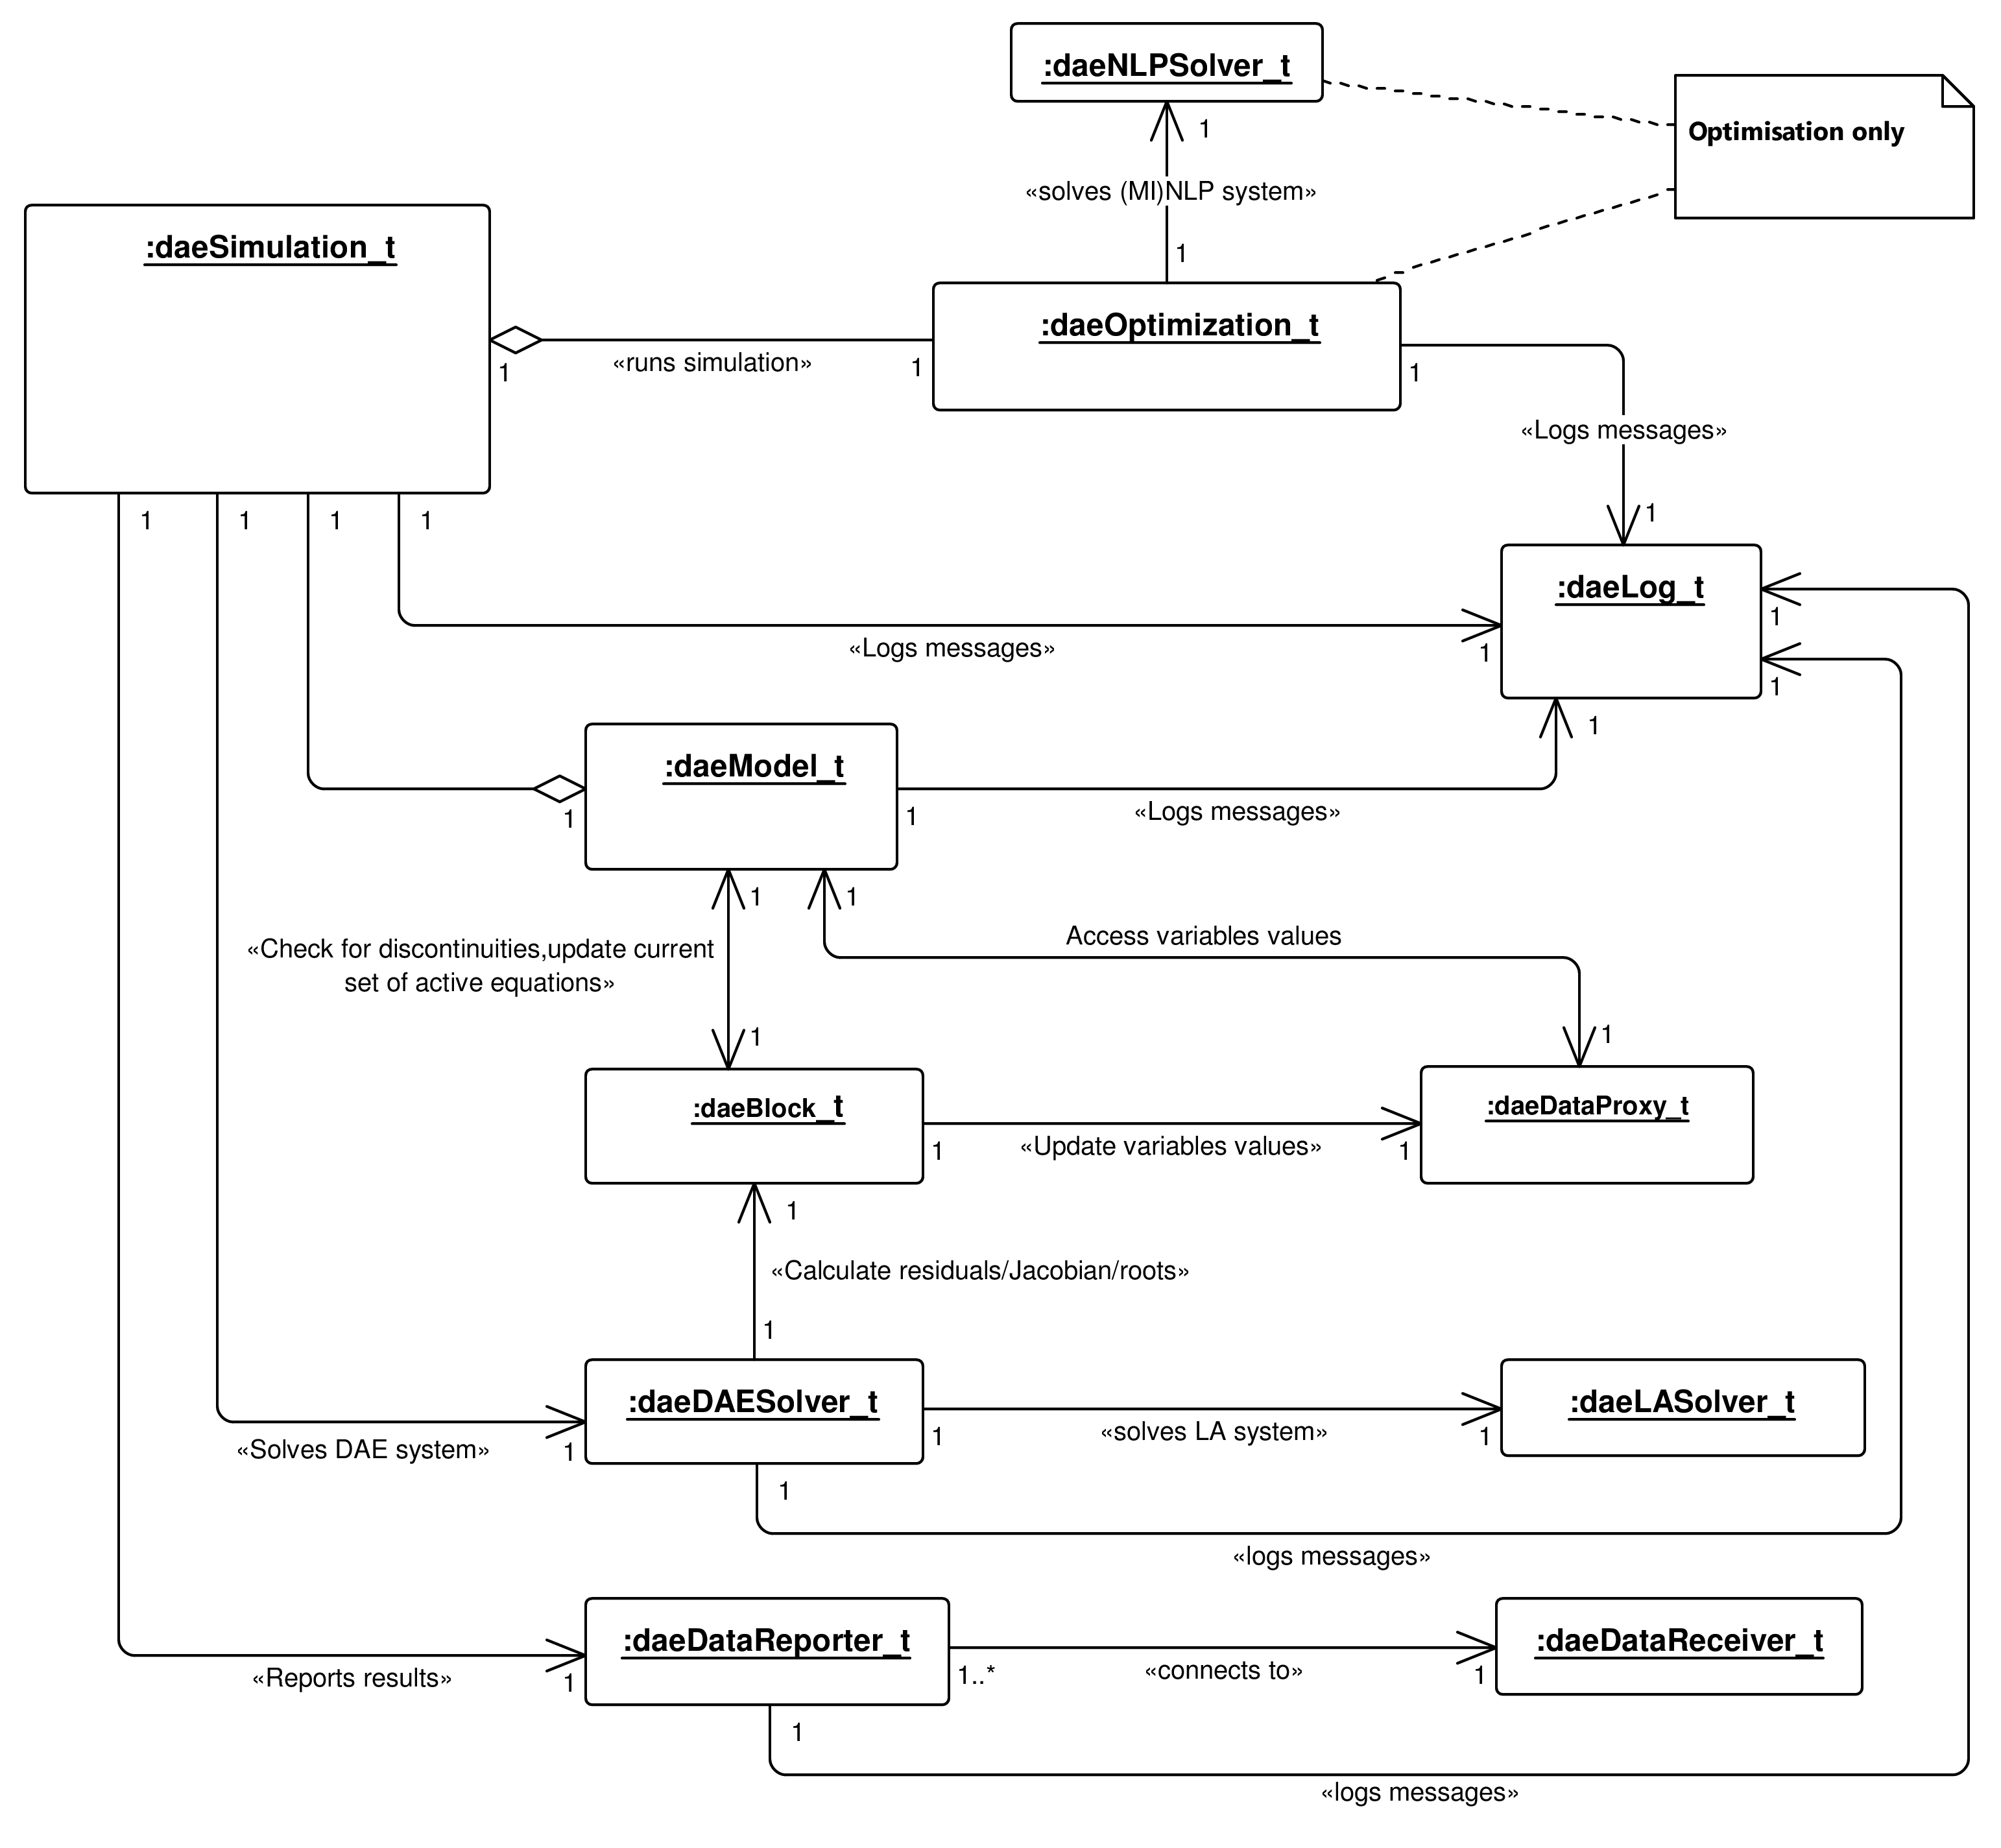
\includegraphics[width=0.68\paperwidth]{daetools-architecture.png}      
               \caption{The architecture of \alert{DAE Tools}.}
            \end{figure}
         \end{center}
     \end{column}
   \end{columns}
\end{frame}

\begin{frame}{Package \textsc{core}}
\scriptsize
{
\begin{table}
  \caption*{The key modelling concepts in the \alert{core} package.}
  \begin{tabularx}{\linewidth}{l>{\raggedright}X}
    \toprule
    \textcolor{sthlmRed}{\textbf{Concept}} & \textcolor{sthlmRed}{\textbf{Description}} \tabularnewline
    \midrule
    \textcolor{sthlmRed}{\textit{daeVariableType\_t}} & Defines a variable type that has the units, lower and upper bounds, a default value and 
                                  an absolute tolerance \tabularnewline
    \textcolor{sthlmRed}{\textit{daeDomain\_t}} & Defines ordinary arrays or spatial distributions such as structured and unstructured grids \tabularnewline 
    \textcolor{sthlmRed}{\textit{daeParameter\_t}} & Defines time invariant quantities that do not change during a simulation \tabularnewline 
    \textcolor{sthlmRed}{\textit{daeVariable\_t}} & Defines time varying quantities that change during a simulation \tabularnewline 
    \textcolor{sthlmRed}{\textit{daePort\_t}} & Defines connection points between model instances for exchange of continuous quantities \tabularnewline 
    \textcolor{sthlmRed}{\textit{daeEventPort\_t}} & Defines connection points between model instances for exchange of discrete messages/events \tabularnewline
    \bottomrule
  \end{tabularx}
\end{table}
}
\end{frame}

\begin{frame}{Package \textsc{core} (cont'd)}
\scriptsize
{
\begin{table}
  \caption*{The key modelling concepts in the \alert{core} package (cont'd).}
  \begin{tabularx}{\linewidth}{l>{\raggedright}X}
    \toprule
    \textcolor{sthlmRed}{\textbf{Concept}} & \textcolor{sthlmRed}{\textbf{Description}} \tabularnewline
    \midrule
    \textcolor{sthlmRed}{\textit{daePortConnection\_t}} & Defines connections between two ports \tabularnewline 
    \textcolor{sthlmRed}{\textit{daeEventPortConnection\_t}} & Defines connections between two event ports \tabularnewline
    \textcolor{sthlmRed}{\textit{daeEquation\_t}} & Defines model equations given in an implicit form \tabularnewline 
    \textcolor{sthlmRed}{\textit{daeSTN\_t}} & Defines state transition networks used to model discontinuous equations \tabularnewline
    \textcolor{sthlmRed}{\textit{daeOnConditionActions\_t}} & Defines actions to be performed when a specified condition is satisfied \tabularnewline
    \textcolor{sthlmRed}{\textit{daeOnEventActions\_t}} & Defines actions to be performed when an event is triggered on the specified event port \tabularnewline
    \textcolor{sthlmRed}{\textit{daeState\_t}} & Defines a state in a state transition network \tabularnewline 
    \textcolor{sthlmRed}{\textit{daeModel\_t}} & Represents a model \tabularnewline
    \bottomrule
  \end{tabularx}
\end{table}
}
\end{frame}

\begin{frame}{Package \textsc{core} - interface implementations}
    \begin{center}
        \begin{figure}
            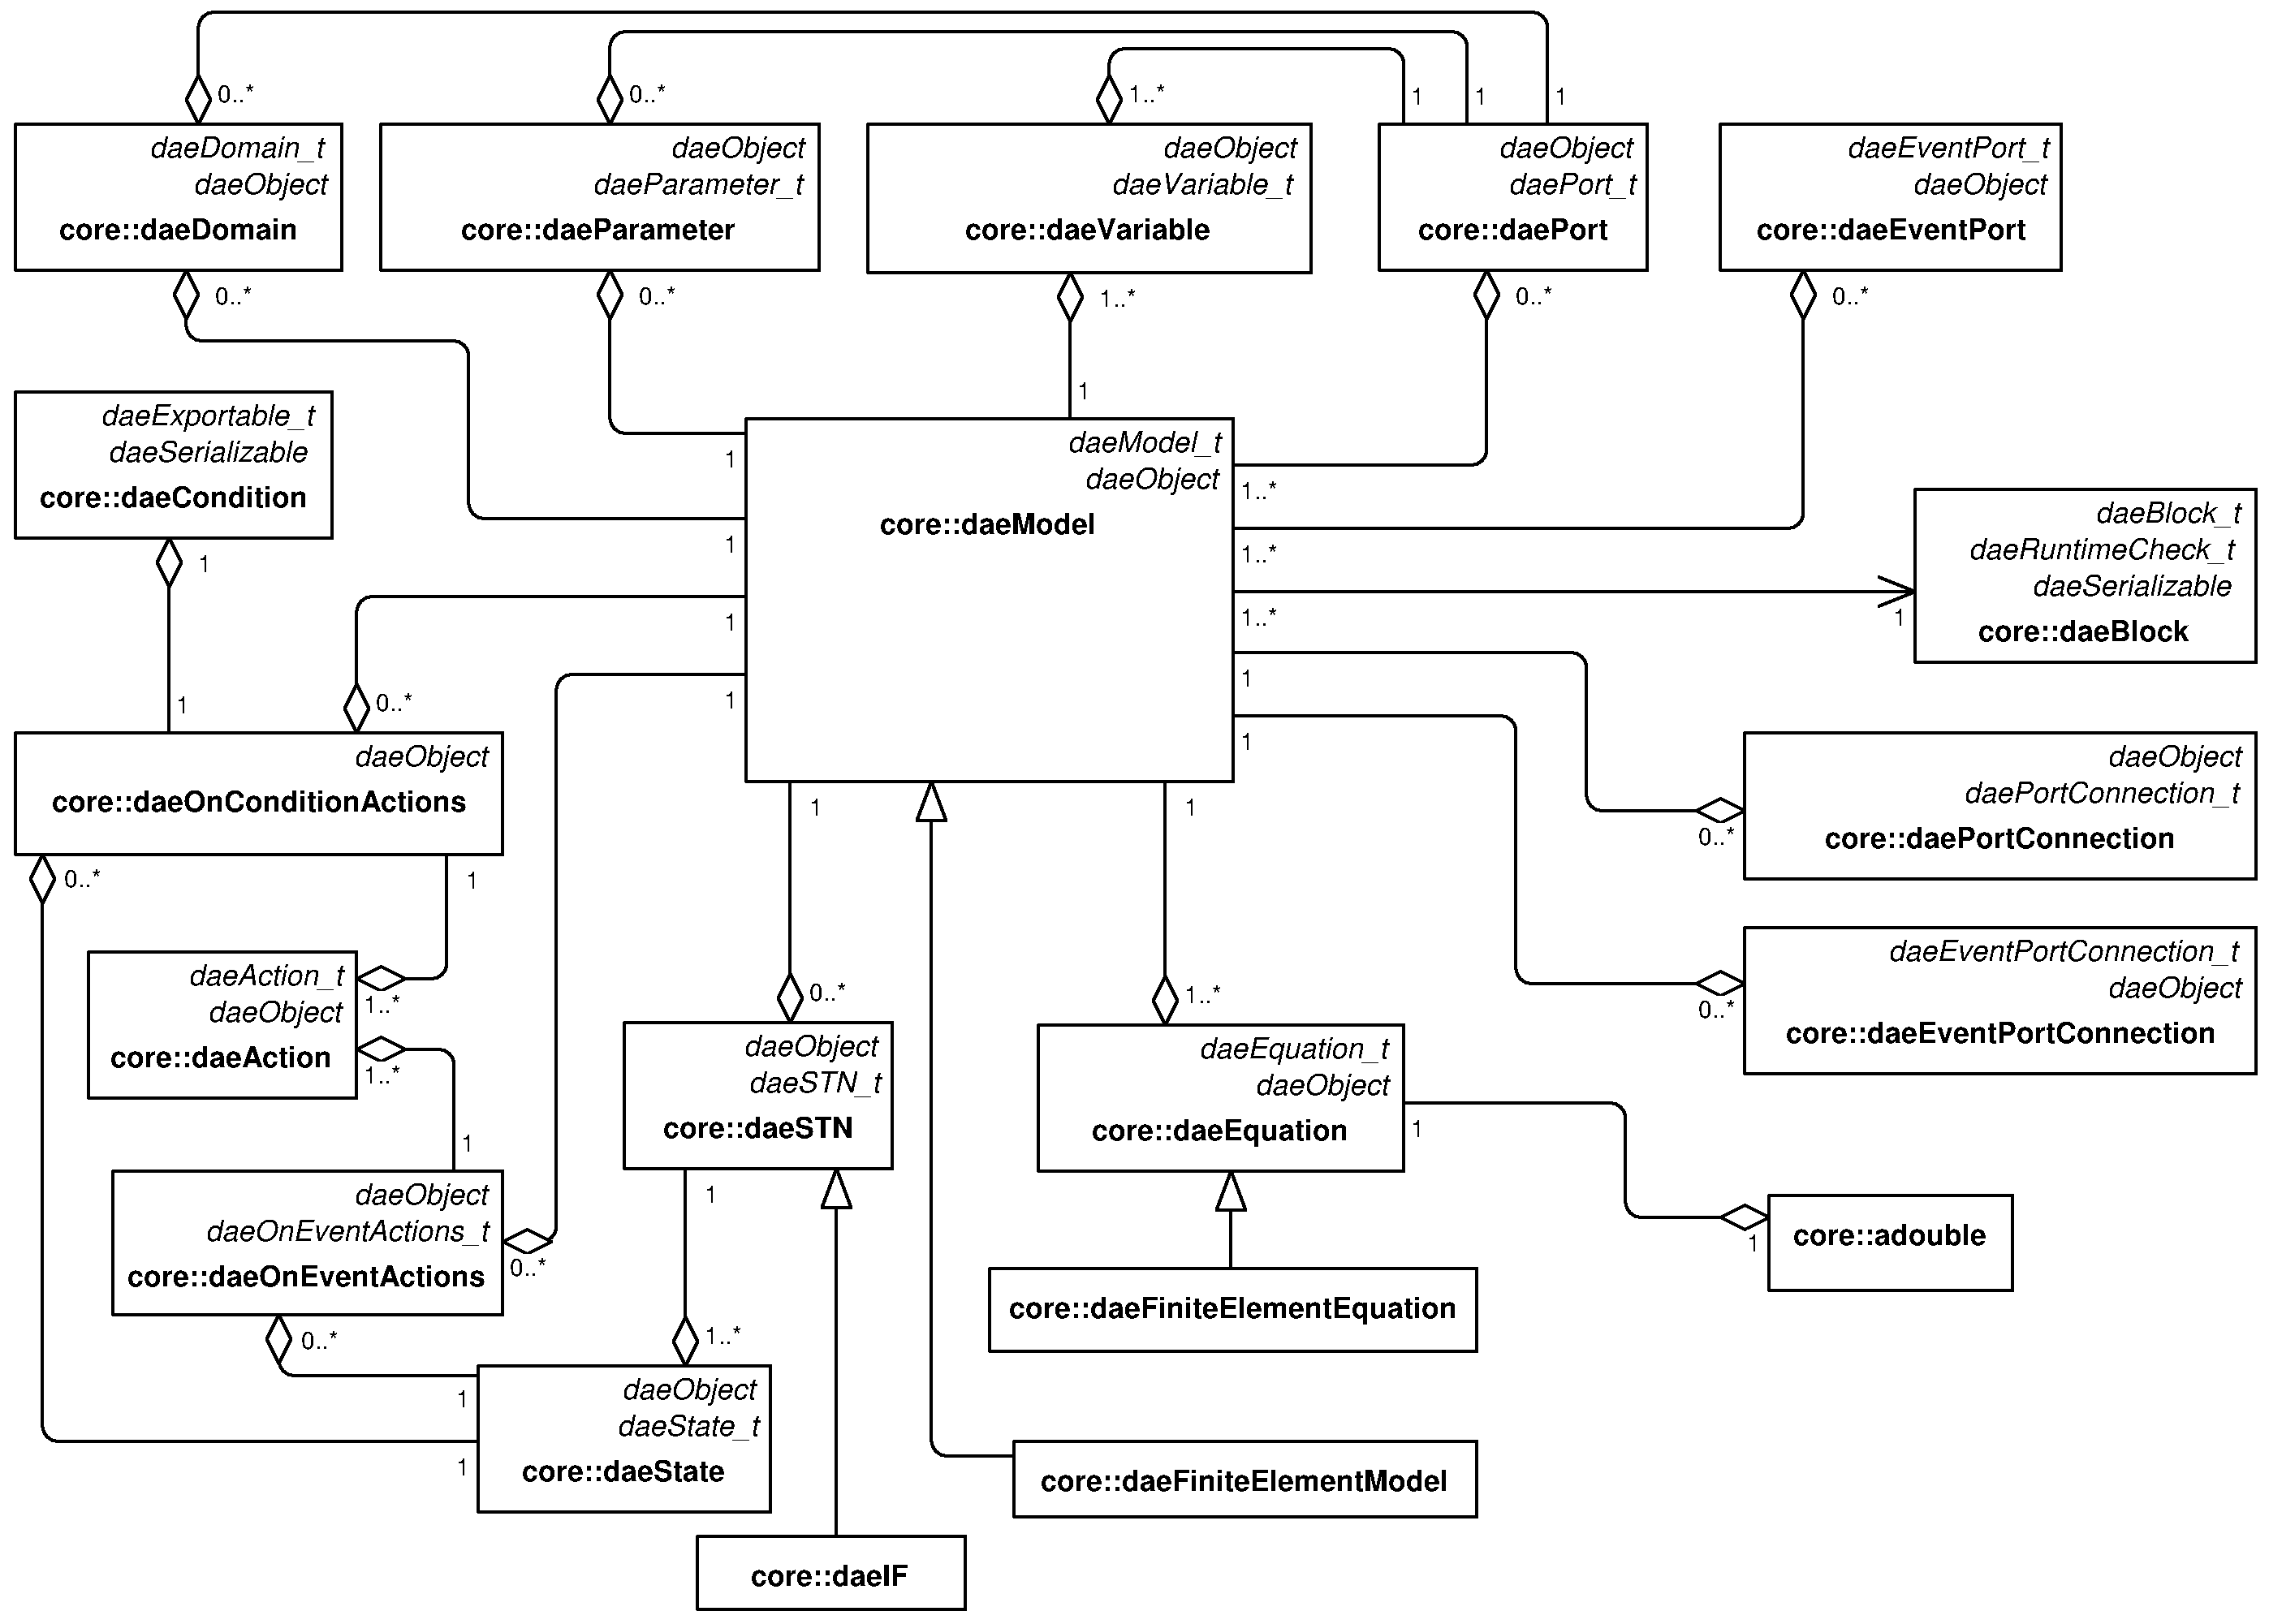
\includegraphics[width=0.8\paperwidth]{Supplemental_Figure_S3.png}      
            %\caption{\alert{core} package interface implementations.}
        \end{figure}
    \end{center}
\end{frame}

\begin{frame}{Package \textsc{activity}}
\scriptsize
{
\begin{table}
  \caption*{The key concepts in the \alert{activity} package.}
  \begin{tabularx}{\linewidth}{l>{\raggedright}X}
    \toprule
    \textcolor{sthlmRed}{\textbf{Concept}} & \textcolor{sthlmRed}{\textbf{Description}} \tabularnewline
    \midrule
    \textcolor{sthlmRed}{\textit{daeSimulation\_t}} & Defines a functionality used to perfom simulations \tabularnewline 
    \textcolor{sthlmRed}{\textit{daeOptimisation\_t}} & Defines a functionality used to perform optimisations \tabularnewline
    \bottomrule
  \end{tabularx}
\end{table}
}
\end{frame}

\begin{frame}{Package \textsc{solvers}}
\scriptsize
{
\begin{table}
  \caption*{The key concepts in the \alert{solvers} package.}
  \begin{tabularx}{\linewidth}{l>{\raggedright}X}
    \toprule
    \textcolor{sthlmRed}{\textbf{Concept}} & \textcolor{sthlmRed}{\textbf{Description}} \tabularnewline
    \midrule
    \textcolor{sthlmRed}{\textit{daeDAESolver\_t}} & Defines a functionality for the solution of DAE systems \tabularnewline 
    \textcolor{sthlmRed}{\textit{daeLASolver\_t}} & Defines a functionality for the solution of LA systems \tabularnewline
    \textcolor{sthlmRed}{\textit{daeNLPSolver\_t}} & Defines a functionality for the solution of (MI)NLP problems \tabularnewline
    \textcolor{sthlmRed}{\textit{daeIDALASolver\_t}} & Sundials IDAS LA solver interface \tabularnewline
    \midrule
    \textcolor{sthlmRed}{\textit{daeMatrix\_t<typename FLOAT>}} & Defines a common matrix functionality \tabularnewline
    \bottomrule
  \end{tabularx}
\end{table}
}
\end{frame}

\begin{frame}{Package \textsc{solvers} - interface implementations}
    \begin{center}
        \begin{figure}
            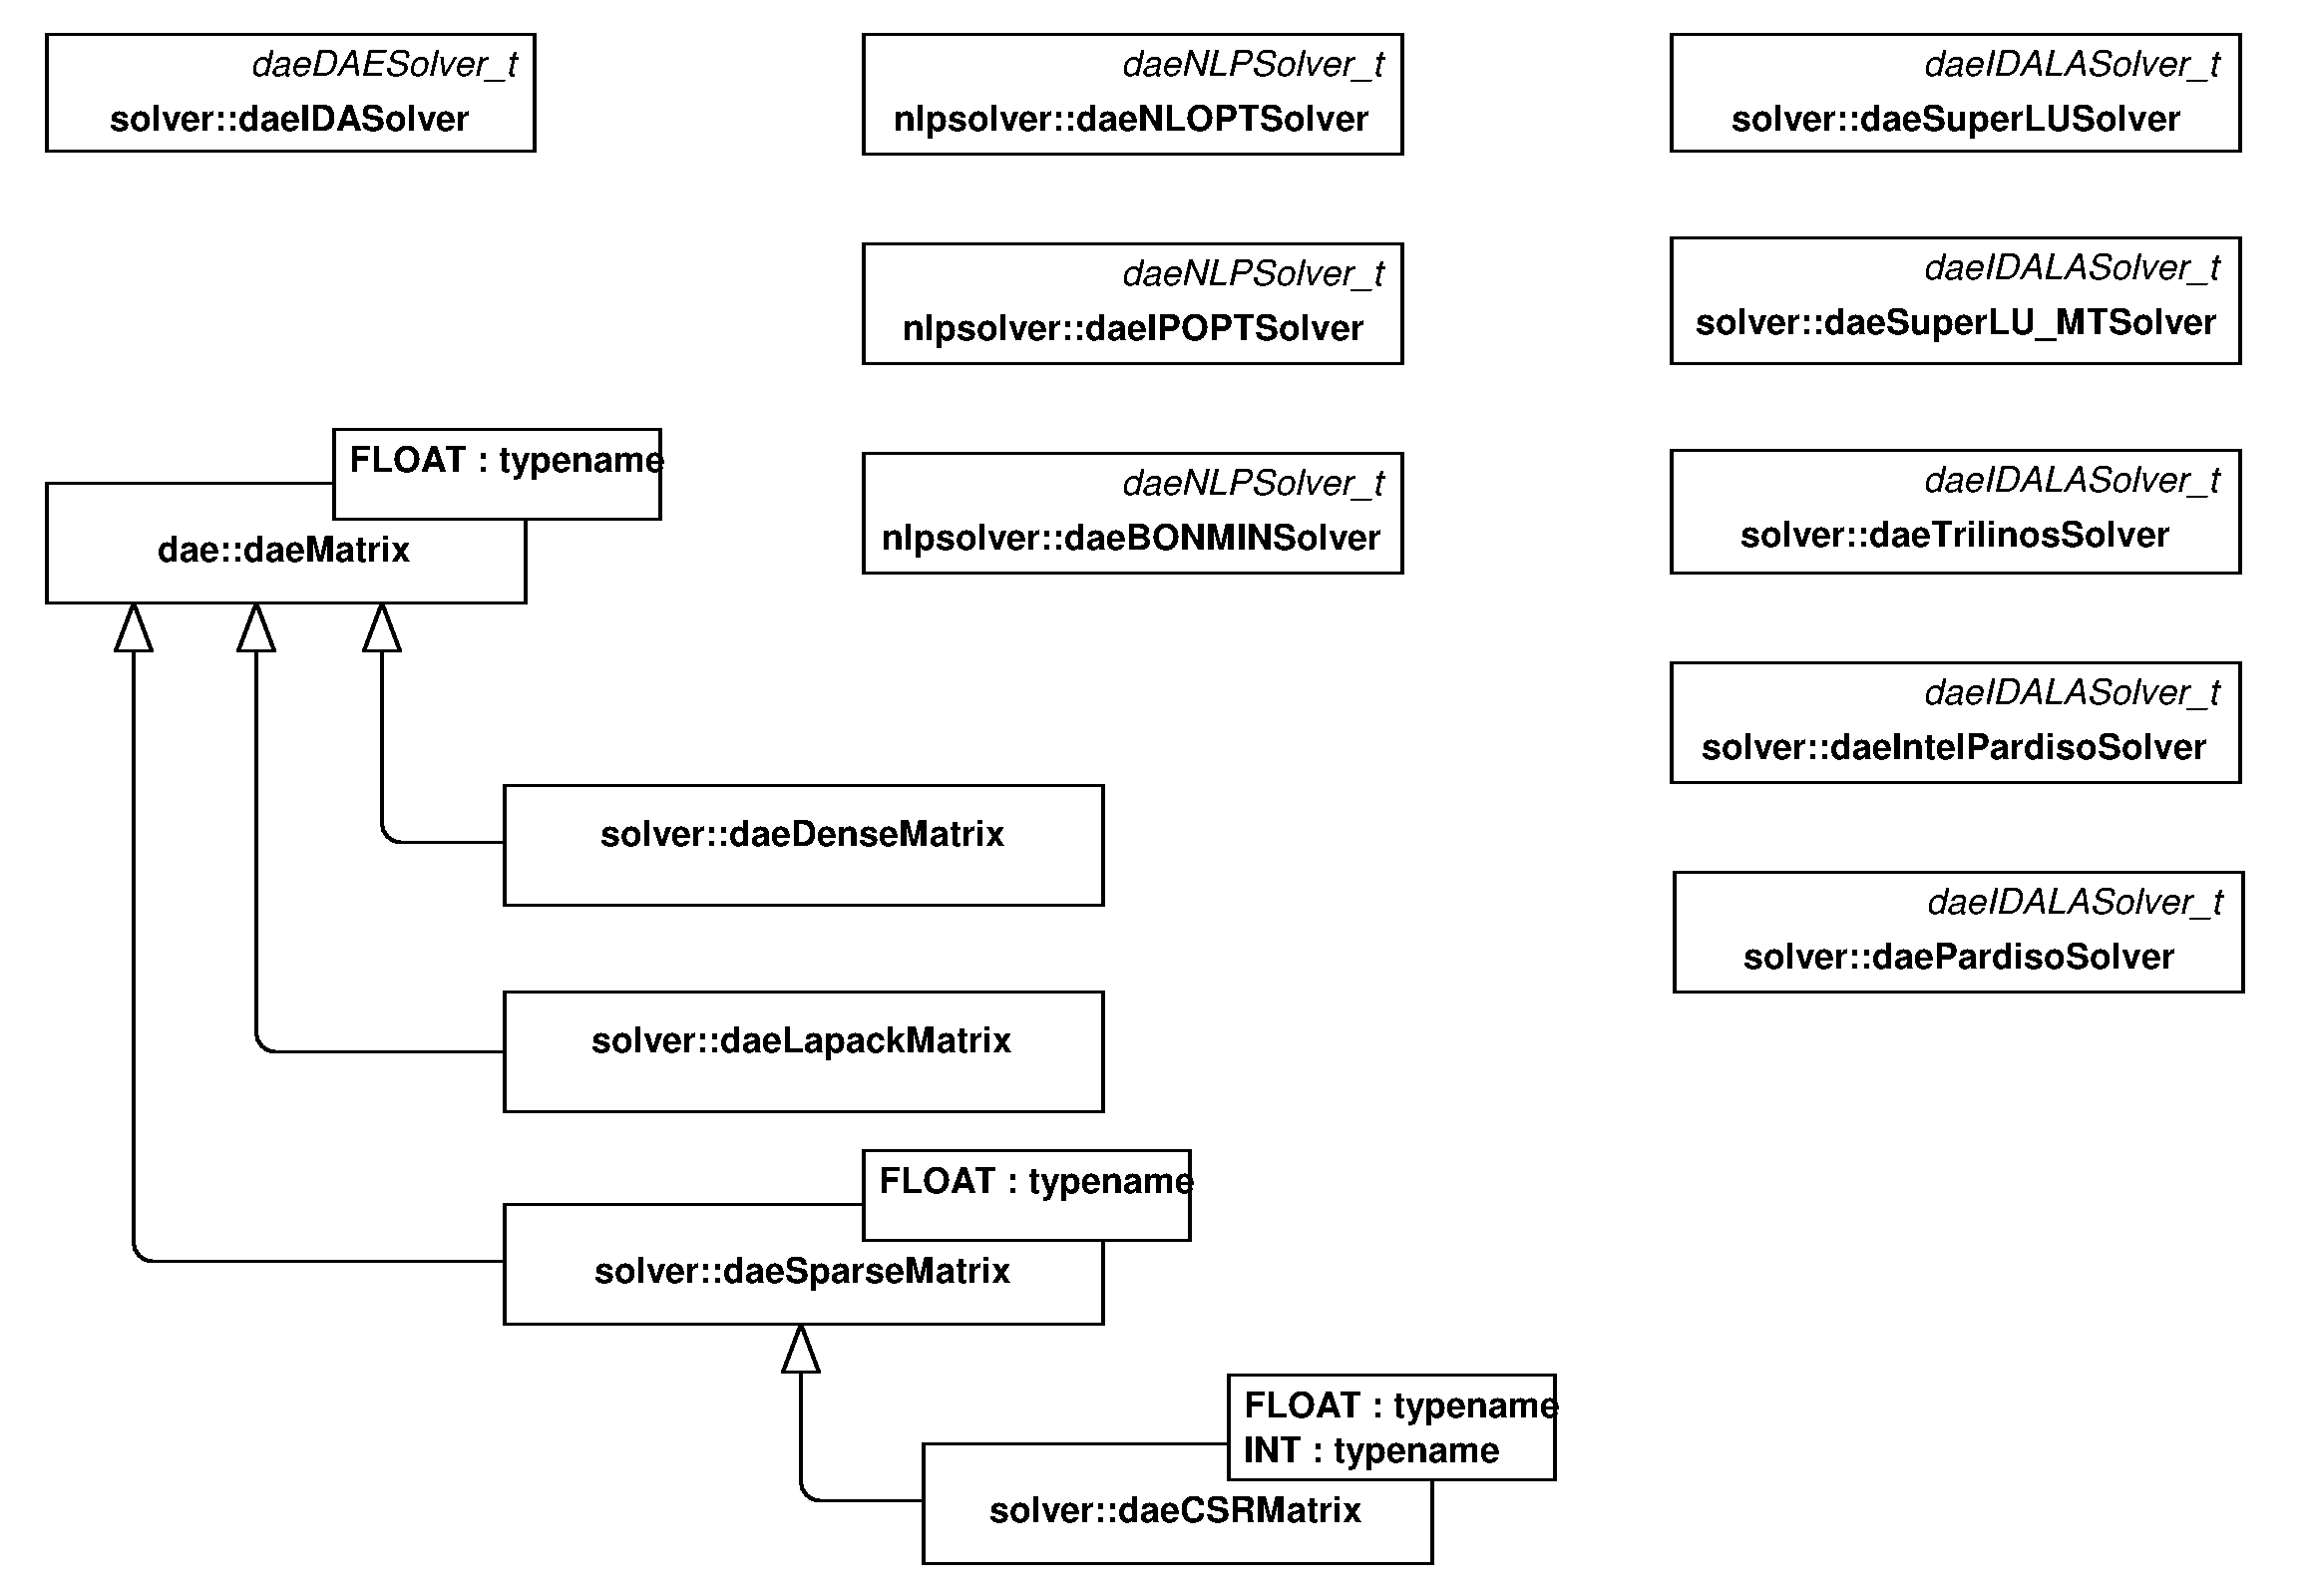
\includegraphics[width=0.75\paperwidth]{Supplemental_Figure_S5.png}      
            %\caption{\alert{solvers} package interface implementations.}
        \end{figure}
    \end{center}
\end{frame}

\begin{frame}{Package \textsc{datareporting}}
\scriptsize
{
\begin{table}
  \caption*{The key concepts in the \alert{datareporting} package.}
  \begin{tabularx}{\linewidth}{l>{\raggedright}X}
    \toprule
    \textcolor{sthlmRed}{\textbf{Concept}} & \textcolor{sthlmRed}{\textbf{Description}} \tabularnewline
    \midrule
    \textcolor{sthlmRed}{\textit{daeDataReporter\_t}} & Defines a functionality/data structures used by a simulation to report the simulation results \tabularnewline 
    \textcolor{sthlmRed}{\textit{daeDataReceiver\_t}} & Defines a functionality/data structures for accessing the simulation results \tabularnewline
    \bottomrule
  \end{tabularx}
\end{table}
}
\end{frame}

\begin{frame}{Package \textsc{datareporting} - interface implementations}
    \begin{center}
        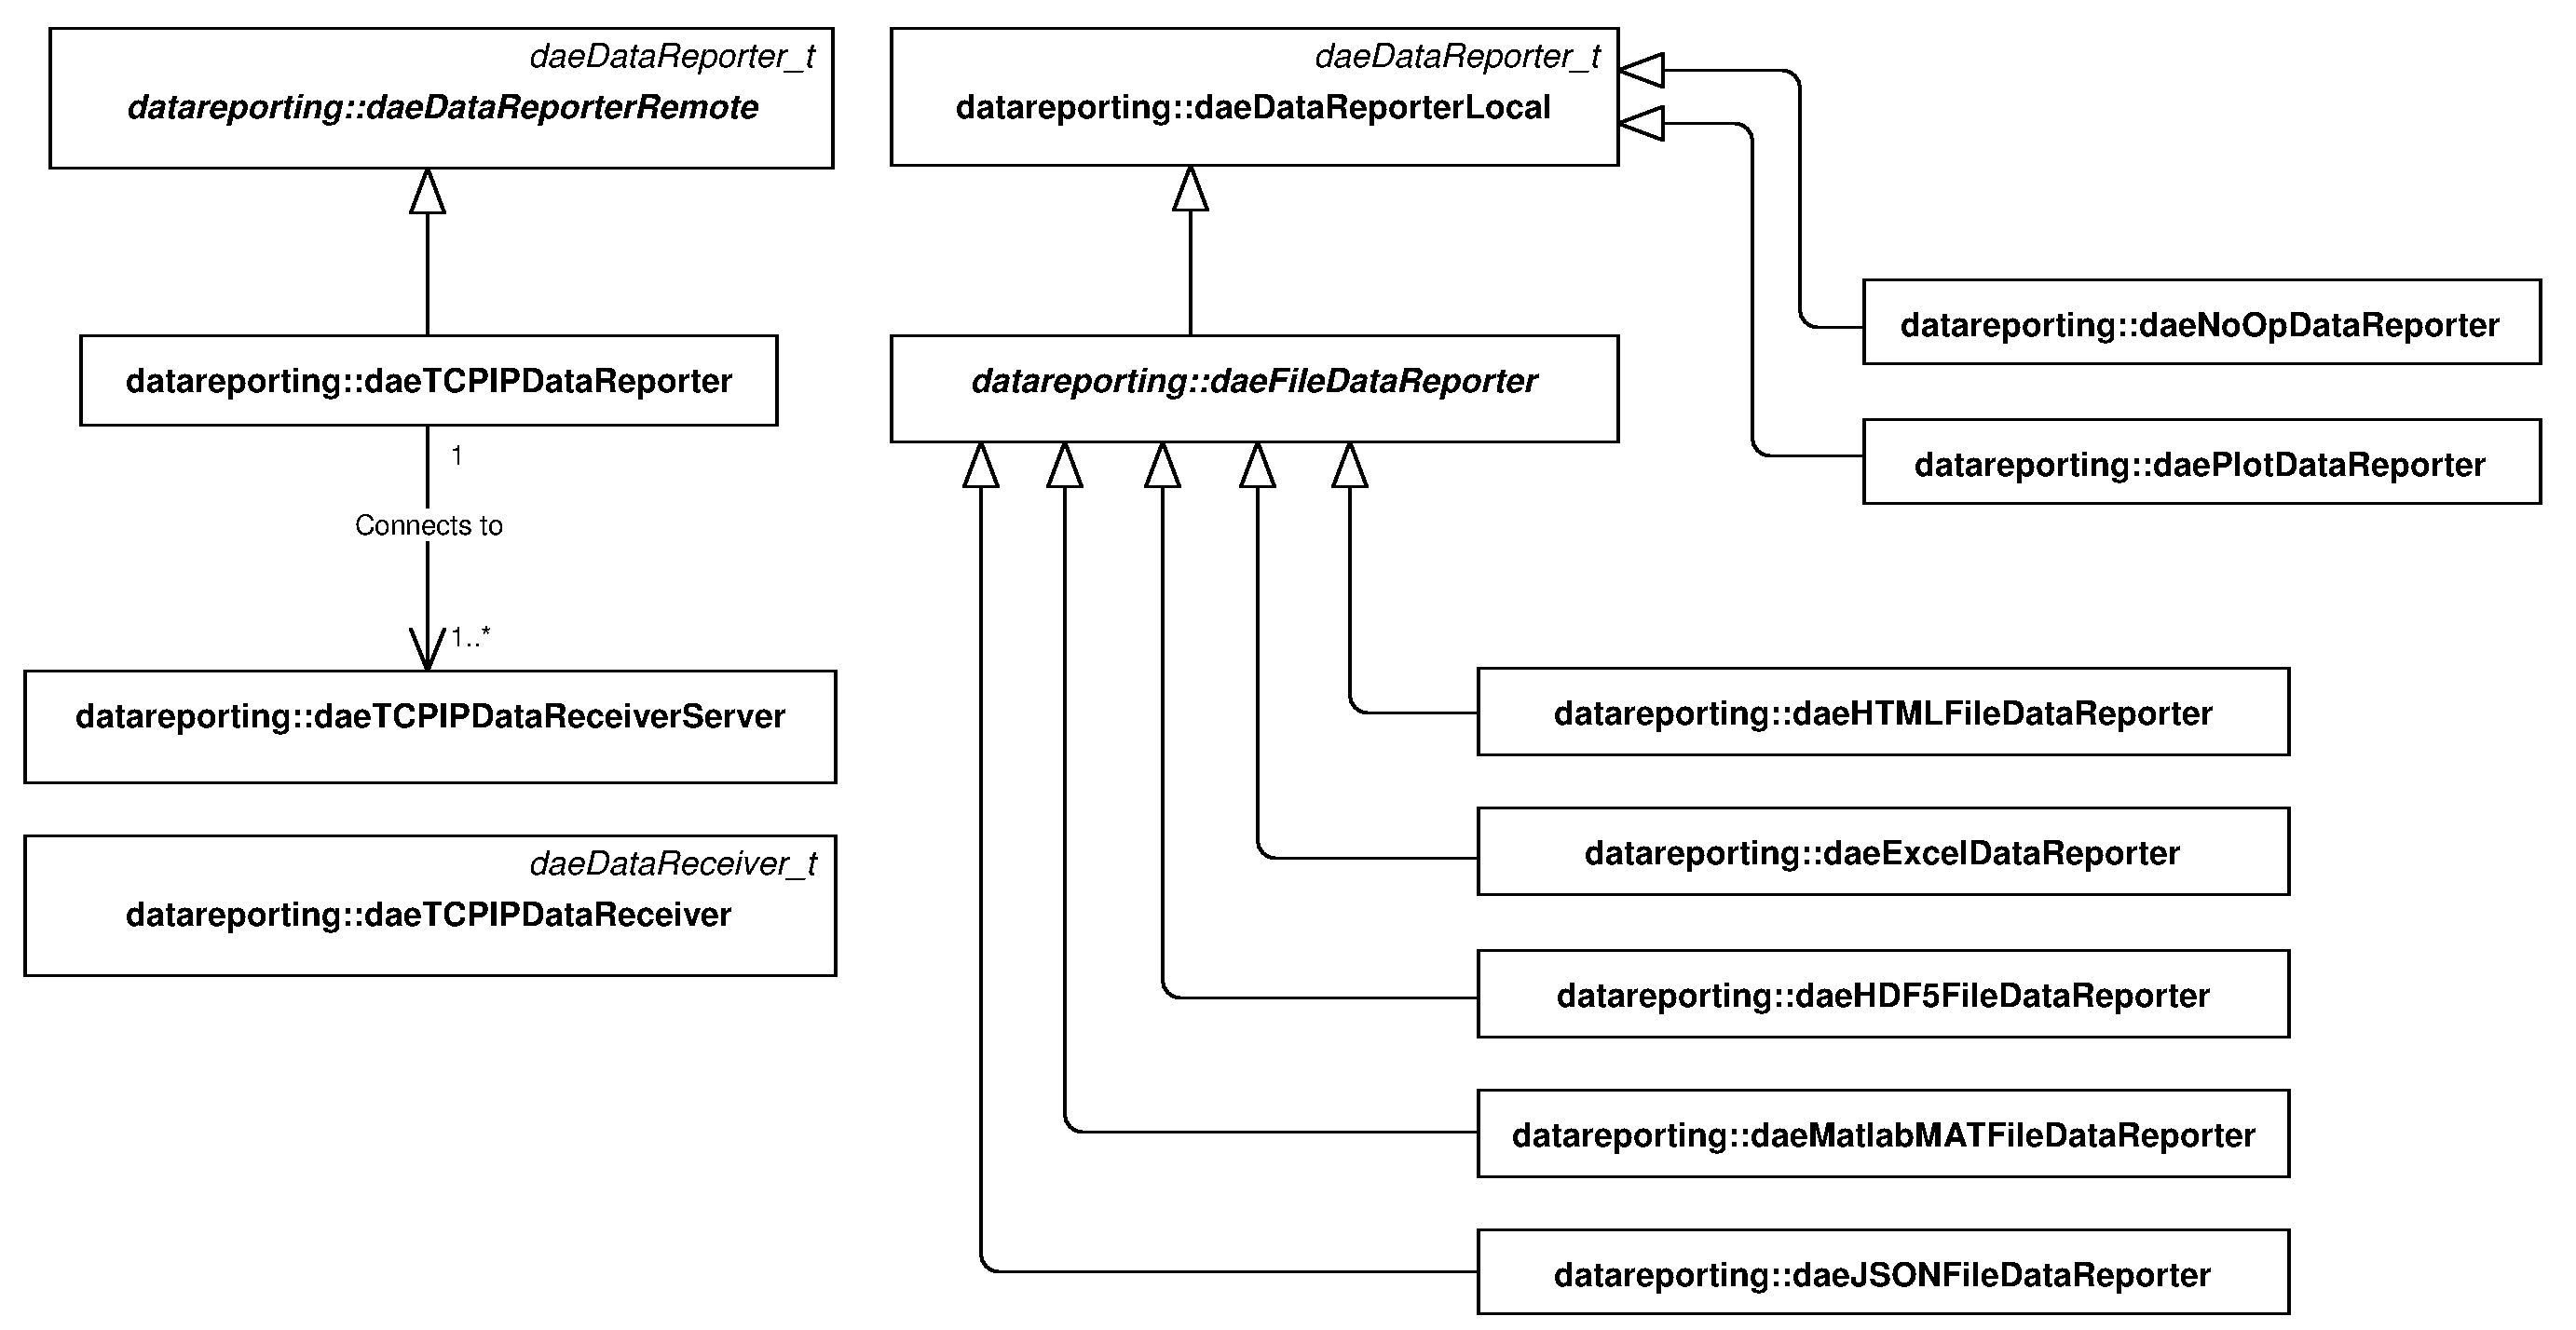
\includegraphics[width=0.8\paperwidth]{Supplemental_Figure_S6.png}      
    \end{center}
\end{frame}

\begin{frame}{Package \textsc{log} and its interface implementations}
\scriptsize
{
\begin{table}
  \caption*{The key concepts in the \alert{log} package.}
  \begin{tabularx}{\linewidth}{l>{\raggedright}X}
    \toprule
    \textcolor{sthlmRed}{\textbf{Concept}} & \textcolor{sthlmRed}{\textbf{Description}} \tabularnewline
    \midrule
    \textcolor{sthlmRed}{\textit{daeLog\_t}} & Defines a functionality for sending messages from a simulation \tabularnewline 
    \bottomrule
  \end{tabularx}
\end{table}
}
    \begin{center}
        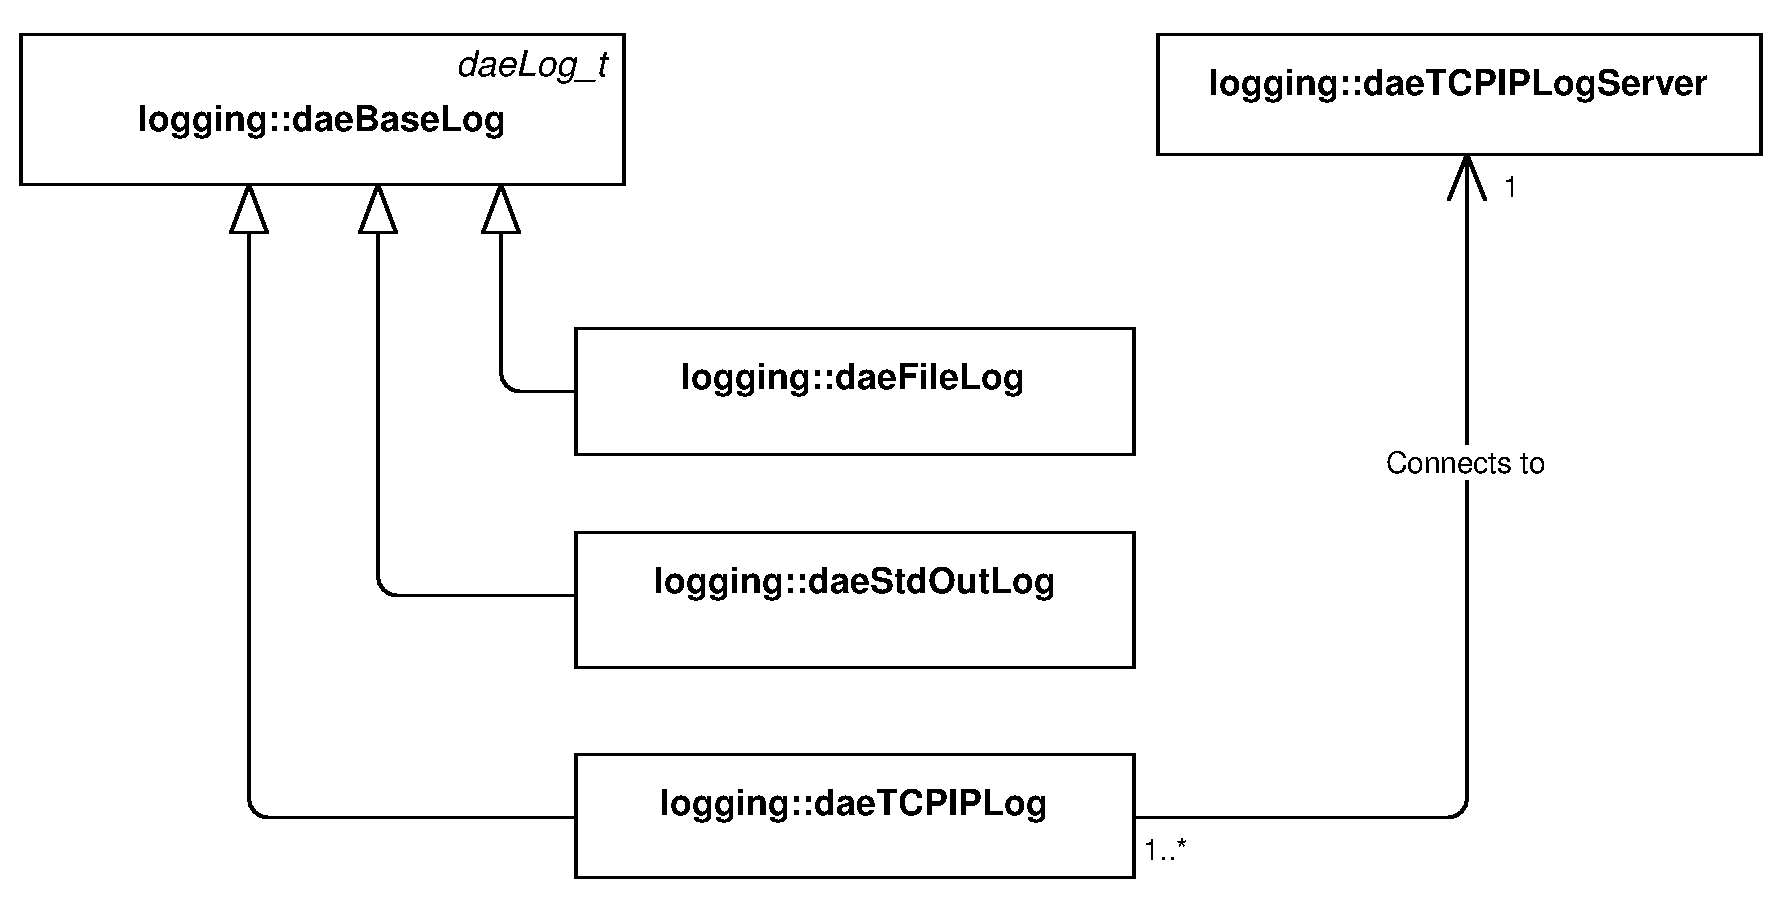
\includegraphics[width=0.6\paperwidth]{Supplemental_Figure_S7.png}      
    \end{center}
\end{frame}

\begin{frame}{Package \textsc{units}}
\scriptsize
{
\begin{table}
  \caption*{The key concepts in the \alert{units} package.}
  \begin{tabularx}{\linewidth}{l>{\raggedright}X}
    \toprule
    \textcolor{sthlmRed}{\textbf{Concept}} & \textcolor{sthlmRed}{\textbf{Description}} \tabularnewline
    \midrule
    \textcolor{sthlmRed}{\textit{unit}} & Defines SI base/derived units \tabularnewline 
    \textcolor{sthlmRed}{\textit{quantity}} & Defines a numerical value in terms of a unit of measurement \tabularnewline
    \bottomrule
  \end{tabularx}
\end{table}
}
\end{frame}

% \section{Developing models with DAE Tools} 
% 
% \begin{frame}{Overview}
% \end{frame}
% 
\section{Use Cases} 

\begin{frame}[plain]{Use Case 1 - Chemical Engineering}
    \begin{itemize}
       {\small
          \item \alert{Continuously Stirred Tank Reactor} (Van de Vusse)
                \href{https://doi.org/10.1021/i160048a700}{[ref]} \href{http://daetools.com/docs/tutorials-chemeng.html\#tutorial-che-1}{[code]}
          \item \alert{Plug Flow Reactor}
                \href{http://daetools.com/docs/tutorials-chemeng.html\#tutorial-che-7}{[code]}
          \item \alert{Distillation column}
                \href{http://dx.doi.org/10.1016/S0098-1354(02)00120-5}{[ref]} \href{http://daetools.com/docs/tutorials-chemeng.html\#tutorial-che-2}{[code]}
          \item \alert{Batch crystalliser}
                \href{http://dx.doi.org/10.1016/j.jcrysgro.2011.06.016}{[ref]} \href{http://daetools.com/docs/tutorials-chemeng.html\#tutorial-che-3}{[code]}
          \item \alert{Discretised Population Balance equations}
                \href{http://dx.doi.org/10.20944/preprints201611.0012.v1}{[ref]} \href{http://daetools.com/docs/tutorials-chemeng.html\#tutorial-che-4}{[code1]}
                \href{http://daetools.com/docs/tutorials-chemeng.html\#tutorial-che-5}{[code2]}
          \item \alert{Newman Porous Electrode Theory} (PET) 
                \href{http://dx.doi.org/10.1007/0-306-47508-1_13}{[ref]} \href{http://daetools.com/docs/tutorials-chemeng.html\#tutorial-che-6}{[code1]}
                \href{https://github.com/raybsmith/daetools-example-battery}{[code2]}
          \item \alert{Multiphase Porous Electrode Theory} (MPET)
                \href{https://arxiv.org/abs/1702.08432}{[ref]} \href{https://bitbucket.org/bazantgroup/mpet}{[code]}
          \item \alert{Hydroxide Exchange Membrane Fuel Cells} (HEMFCs)
                \href{http://doi.org/10.1038/nnano.2016.265}{[ref]}
          \item \alert{Maxwell-Stefan equations} (porous membranes)
                \href{http://doi.org/10.1007/s10450-015-9670-z}{[ref]} \href{http://daetools.com/docs/tutorials-chemeng.html\#tutorial-che-8}{[code]}
          \item \alert{Presssure Swing Adsorption}
                \href{http://doi.org/10.1021/ie801357a}{[ref1]} \href{http://doi.org/10.1021/ie0712582}{[ref2]}
       }
    \end{itemize}
\end{frame}

\begin{frame}[plain]{Use Case 2 - Finite Element Method}
    \begin{itemize}
      {\small
          \item \alert{Transient heat conduction/convection}
                \href{http://daetools.com/docs/tutorials-fe.html\#tutorial-dealii-2}{[code]}
          \item \alert{Cahn-Hilliard equation}
                \href{http://daetools.com/docs/tutorials-fe.html\#tutorial-dealii-3}{[code]}
          \item \alert{Flow through the porous media}
                \href{http://daetools.com/docs/tutorials-fe.html\#tutorial-dealii-5}{[code]}
          \item \alert{Diffusion/reaction in an irregular catalyst shape}
                \href{http://daetools.com/docs/tutorials-fe.html\#tutorial-dealii-6}{[code]}
      }
    \end{itemize}
    \begin{center}
        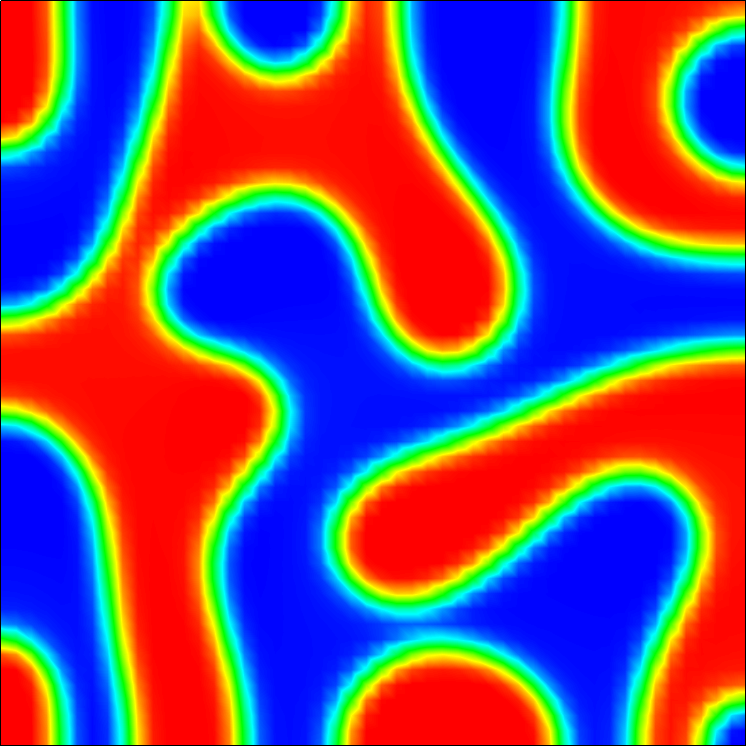
\includegraphics[align=c, height=0.35\textheight]{cahn-hilliard.png}
        \;
        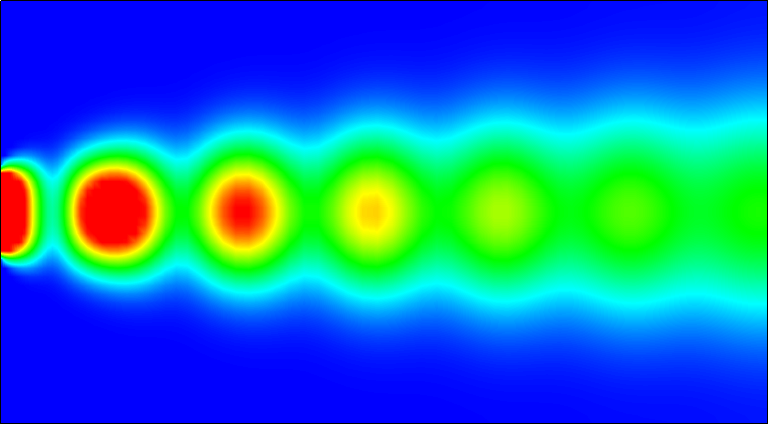
\includegraphics[align=c, height=0.35\textheight]{heat_convection.png}
    \end{center}
\end{frame}

\begin{frame}[plain]{Use Case 3 - Parameter Estimation \& Optimal Control}
    \begin{center}
        {\small
            \alert{Large-scale Constrained Optimization Problem Set (COPS)}
        }
    \end{center}  
    \begin{itemize}
      {\small
          \item Determination of the reaction coefficients in the thermal isomerization of $\alpha$-pinene (COPS 5)
                \href{http://daetools.com/docs/tutorials-chemeng-optimisation.html\#tutorial-che-opt-2}{[code]}
          \item Determination of stage specific growth and mortality rates for species at each stage as a function of time (COPS 6)
                \href{http://daetools.com/docs/tutorials-chemeng-optimisation.html\#tutorial-che-opt-3}{[code]}
          \item Determination of the reaction coefficients for the catalytic cracking of gas oil and other byproducts (COPS 12)
                \href{http://daetools.com/docs/tutorials-chemeng-optimisation.html\#tutorial-che-opt-4}{[code]}
          \item Determination of the reaction coefficients for the conversion of methanol into various hydrocarbons (COPS 13)
                \href{http://daetools.com/docs/tutorials-chemeng-optimisation.html\#tutorial-che-opt-5}{[code]}
          \item Catalyst mixing in a tubular plug flow reactor (COPS 14)
                \href{http://daetools.com/docs/tutorials-chemeng-optimisation.html\#tutorial-che-opt-6}{[code]}
      }
    \end{itemize}
\end{frame}


\begin{frame}[plain]{Use Case 4 - Multi-scale modelling}
    \begin{center}
        \alert{Multi-scale model of phase-separating battery electrodes}
        \footnote{\tiny{Li et al. (2014) \textit{Current-induced transition
                    from particle-by-particle to concurrent intercalation in phase-separating battery electrodes}.
                    Nature Materials 13(12):1149–1156. \href{https://doi.org/10.1038/nmat4084}{doi:10.1038/nmat4084.}}
                }
     \end{center}  
    \begin{columns}[c]
      \begin{column}{0.6\textwidth}
        {\small
         \begin{itemize}
            \item Approach: \alert{porous electrode theory}
            \item Lithium transport in:
            \begin{itemize}
                \item Particles (small length scale)
                \item Electrolyte (large length scale)
            \end{itemize}
            \item Two phases are coupled via a volume-averaged approach
            \item Particles act as volumetric source/sink terms as they interact with the
                  electrolyte via reactions
            \item The code available at \alert{\href{https://bitbucket.org/bazantgroup/mpet}{Bitbucket}}
        \end{itemize}
        }
      \end{column}
      
      \begin{column}{0.4\textwidth}
        \begin{center}
          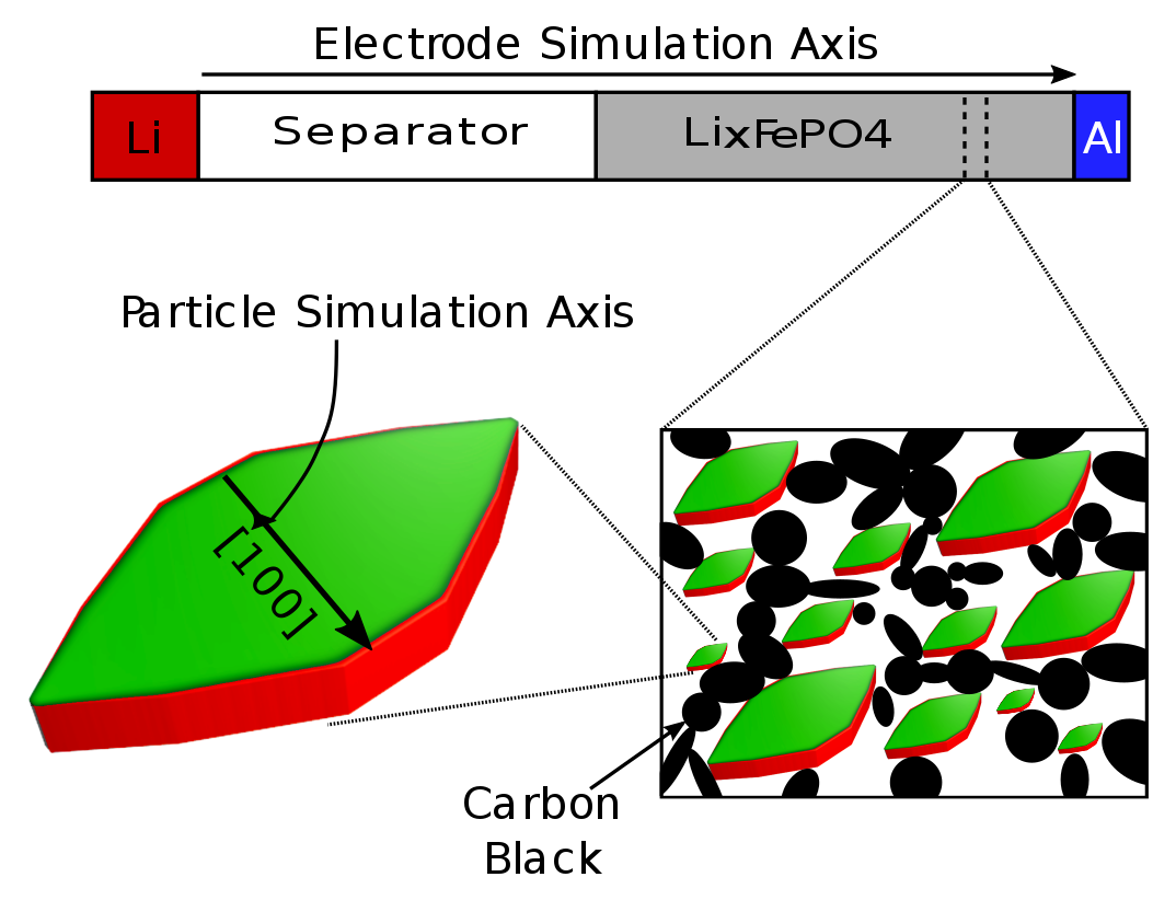
\includegraphics[align=c, width=\textwidth]{multi_scale.png}
        \end{center}
      \end{column}
    \end{columns}
\end{frame}

\begin{frame}{Use Case 4 - Multi-scale modelling (cont'd)}
    \begin{columns}[c]
      \begin{column}{0.55\paperwidth}
        {\scriptsize
         \begin{itemize}
            \item Spatial discretisation: finite-volume method
            \item Large DAE system: 
                \begin{itemize}
                    \scriptsize
                    {
                        \item Discretised transport eqns.
                        \item Algebraic constraints (electrostatic eqns.) 
                        \item Constraints on the current
                    }
                \end{itemize}
            \item Implementations
                \begin{itemize}
                    \scriptsize
                    {
                        \item MATLAB (ode15s solver)
                        \item DAE Tools (Sundials IDAS)
                    }
                \end{itemize}
            \item DAE Tools up to 10x faster (average 4.22x) due to:
                \begin{itemize}
                    \scriptsize
                    {
                        \item Built-in support for auto-differentiation
                        \item Rapid derivative evaluation
                        \item Accurate derivatives
                    }
                \end{itemize}
        \end{itemize}
        }
      \end{column}
      
      \begin{column}{0.40\paperwidth}
        \begin{center}
          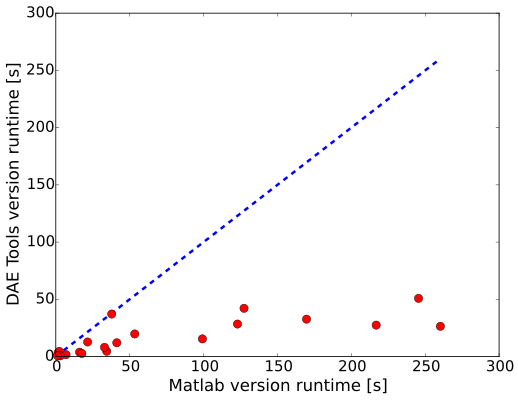
\includegraphics[align=c, width=\textwidth]{parity_plot.png}
        \end{center}
      \end{column}
    \end{columns}
\end{frame}

\begin{frame}[plain]{Use Case 5 - Embedded simulator (back end)}
    \begin{center}
        \alert{Network Interchange format for NEuroscience (NineML)}
    \end{center}   
    \small{XML-based DSL for modelling of networks of spiking neurones 
                \href{http://software.incf.org/software/nineml}{
\includegraphics[align=b, height=0.8em]{link.png}}
                } \linebreak
    \small{DAE Tools embedded into a \alert{reference implementation simulator}}
    \begin{columns}[c]
      \begin{column}{0.50\paperwidth}
        {\scriptsize
         \begin{itemize}
            \item \alert{Abstraction Layer (AL)}
                \begin{itemize}
                    \scriptsize
                    {
                        \item Mathematical description
                        \item Modelling concepts
                    }
                \end{itemize}
            \item \alert{User Layer (UL)}
                \begin{itemize}
                    \scriptsize
                    {
                        \item Parameters values
                        \item Instantiations
                    }
                \end{itemize}
            \item NineML concepts $\rightarrow$ DAE Tools concepts
                \begin{itemize}
                    \scriptsize
                    {
                        \item Neurone models
                        \item Synapse models
                        \item Populations of neurones
                        \item Layers of neurones
                    }
                \end{itemize}
        \end{itemize}
        }
      \end{column}
      
      \begin{column}{0.45\paperwidth}
        \begin{center}
            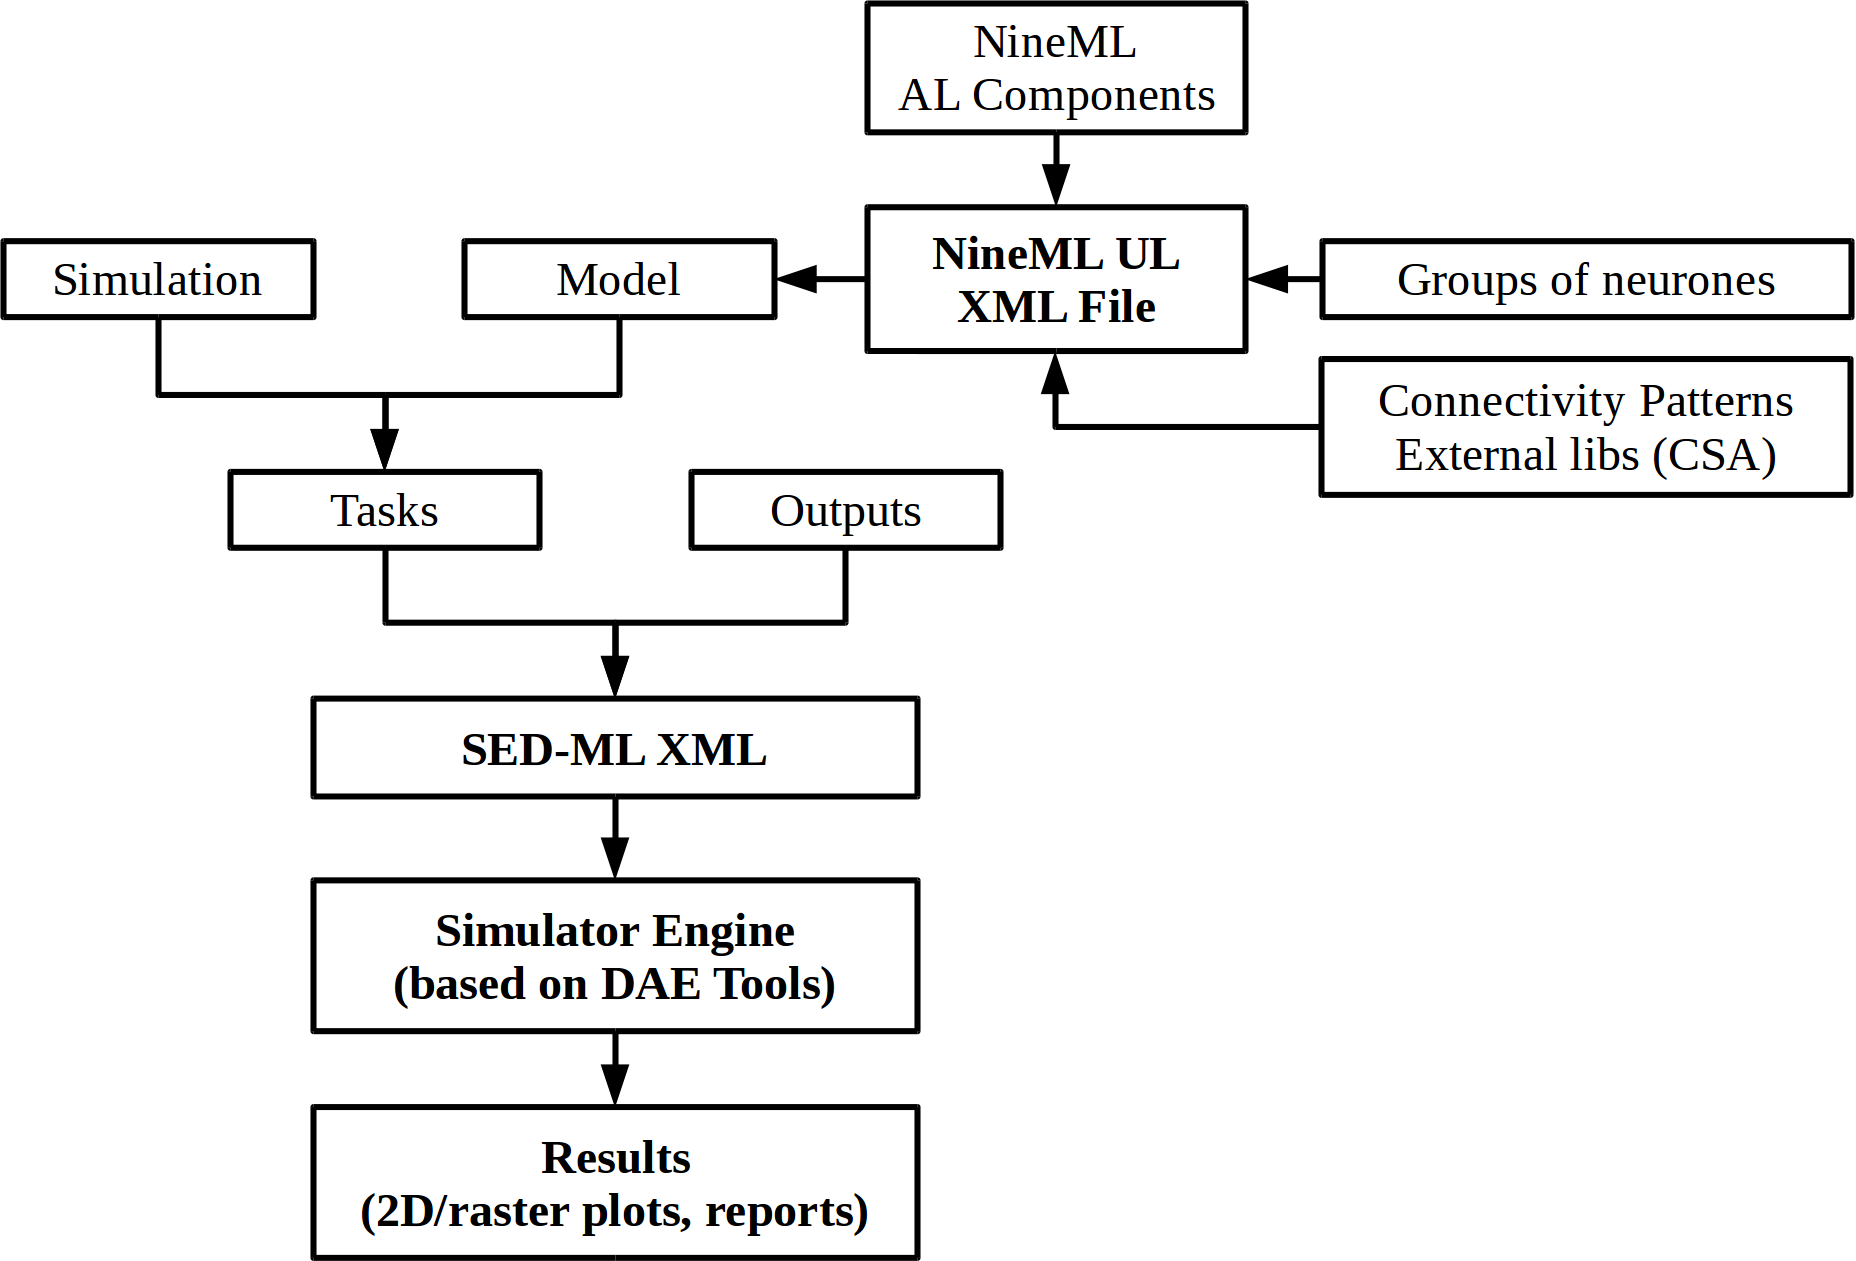
\includegraphics[align=c, width=\textwidth]{nineml_ris.png}
        \end{center}
      \end{column}
    \end{columns}
\end{frame}

\begin{frame}[plain]{Use Case 6 - Web application / Web service}
    \begin{center}
        \alert{Network Interchange format for NEuroscience (NineML)}
    \end{center}   
    \small{DAE Tools serves as \alert{AL components validator/report generator}}
    
    \begin{itemize}
        \item Three flavours:
        \begin{itemize}
            \item \alert{Desktop application} (Python + Qt GUI)
            \item \alert{Web application} (jQuery GUI)
            \item \alert{Web service} with REST API (Apache server + Python WSGI)
        \end{itemize}
        \item Inputs:
            \begin{itemize}
                \item Abstraction Layer component to test
                \item Parameters and inlet ports values, initial conditions
                \item One or more tests (optional)
            \end{itemize}
        \item Outputs:
            \begin{itemize}
                \item Model report (pdf, html)
                \item Test(s) results (variable plots)
            \end{itemize}
    \end{itemize}
\end{frame}

% \appendix
% \begin{frame}[allowframebreaks]{References}
% \begin{thebibliography}{JModelica-2010}
% 
% \bibitem[Akesson et~al., 2010]{JModelica-2010}
% Akesson, J., Arzen, K.-E., Gafvert, M., Bergdahl, T., and Tummescheit, H.
%   (2010).
% \newblock Modeling and optimization with {Optimica} and {JModelica}.org -
%   languages and tools for solving large-scale dynamic optimization problems.
% \newblock {\em Comput. Chem. Eng.}, 34(11):1737--1749.
% 
% \bibitem[Andersson et~al., 2015]{Assimulo-2015}
% Andersson, C., Fuhrer, C., and Akesson, J. (2015).
% \newblock Assimulo: A unified framework for ode solvers.
% \newblock {\em Math. Comput. Simulat.}, 116(0):26 -- 43.
% 
% \bibitem[Balay et~al., 2015]{petsc}
% Balay, S., Abhyankar, S., Adams, M.~F., Brown, J., Brune, P., Buschelman, K.,
%   Dalcin, L., Eijkhout, V., Gropp, W.~D., Kaushik, D., Knepley, M.~G., McInnes,
%   L.~C., Rupp, K., Smith, B.~F., Zampini, S., and Zhang, H. (2015).
% \newblock {PETS}c users manual.
% \newblock Technical Report ANL-95/11 - Revision 3.6, Argonne National
%   Laboratory.
% 
% \bibitem[Barton and Pantelides, 1993]{Barton-and-Pantelides-1993}
% Barton, P.~I. and Pantelides, C.~C. (1993).
% \newblock {gPROMS - A Combined Discrete/Continuous Modelling Environment for
%   Chemical Processing Systems}.
% \newblock {\em Simul. Ser.}, 25:25--34.
% 
% \bibitem[Barton and Pantelides, 1994]{Barton-and-Pantelides-1994}
% Barton, P.~I. and Pantelides, C.~C. (1994).
% \newblock {Modeling of combined discrete/continuous processes}.
% \newblock {\em AIChE J.}, 40(6):966--979.
% 
% \bibitem[Bonami et~al., 2008]{Bonami-etal-2008}
% Bonami, P., Biegler, L.~T., Conn, A.~R., Cornu{\'e}jols, G., Grossmann, I.~E.,
%   Laird, C.~D., Lee, J., Lodi, A., Margot, F., Sawaya, N., and W{\"a}chter, A.
%   (2008).
% \newblock {An algorithmic framework for convex mixed integer nonlinear
%   programs}.
% \newblock {\em Discrete Optim.}, 5(2):186--204.
% \newblock In Memory of George B. Dantzig.
% 
% \bibitem[Brook et~al., 1988]{Brook-etal-1988}
% Brook, A., Kendrick, D., and Meeraus, A. (1988).
% \newblock {GAMS, a User's Guide}.
% \newblock {\em SIGNUM Newsl.}, 23(3-4):10--11.
% 
% \bibitem[Eaton et~al., 2015]{octave}
% Eaton, J., Bateman, D., Hauberg, S., and Wehbring, R. (2015).
% \newblock {\em {GNU Octave} version 4.0.0 manual: a high-level interactive
%   language for numerical computations}.
% 
% \bibitem[Elmqvist, 1978]{Elmqvist-1978}
% Elmqvist, H. (1978).
% \newblock {\em {A Structured Model Language for Large Continuous Systems}}.
% \newblock PhD thesis, Department of Automatic Control, Lund University, Sweden.
% 
% \bibitem[Fritzson et~al., 2005]{OpenModelica-2005}
% Fritzson, P., Aronsson, P., Lundvall, H., Nystrom, K., Pop, A., Saldamli, L.,
%   and Broman, D. (2005).
% \newblock The openmodelica modeling, simulation, and development environment.
% \newblock SIMS - Scandinavian Simulation Society.
% 
% \bibitem[Fritzson and Engelson, 1998]{Fritzson-and-Engelson-1998}
% Fritzson, P. and Engelson, V. (1998).
% \newblock {Modelica --- A unified object-oriented language for system modeling
%   and simulation}.
% \newblock In Jul, E., editor, {\em {ECOOP{\rq}98 --- Object-Oriented
%   Programming}}, volume 1445 of {\em {Lecture Notes in Computer Science}},
%   pages 67--90. Springer Berlin Heidelberg.
% 
% \bibitem[Hedengren et~al., 2014]{APMonitor-2014}
% Hedengren, J.~D., Shishavan, R.~A., Powell, K.~M., and Edgar, T.~F. (2014).
% \newblock Nonlinear modeling, estimation and predictive control in apmonitor.
% \newblock {\em Comput. Chem. Eng.}, 70:133 -- 148.
% \newblock Manfred Morari Special Issue.
% 
% \bibitem[Hindmarsh et~al., 2005]{Hindmarsh-etal-2005}
% Hindmarsh, A.~C., Brown, P.~N., Grant, K.~E., Lee, S.~L., Serban, R., Shumaker,
%   D.~E., and Woodward, C.~S. (2005).
% \newblock {SUNDIALS: Suite of Nonlinear and Differential/Algebraic Equation
%   Solvers}.
% \newblock {\em ACM Trans. Math. Softw.}, 31(3):363--396.
% 
% \bibitem[Johnson, 2015]{nlopt}
% Johnson, S.~G. (2015).
% \newblock {The NLopt nonlinear-optimization package}.
% 
% \bibitem[Li, 2005]{Li-2005}
% Li, X.~S. (2005).
% \newblock {An Overview of SuperLU: Algorithms, Implementation, and User
%   Interface}.
% \newblock {\em ACM Trans. Math. Softw.}, 31(3):302--325.
% 
% \bibitem[Li et~al., 2014]{Li-etal-2014}
% Li, Y., El~Gabaly, F., Ferguson, T.~R., Smith, R.~B., Bartelt, N.~C., Sugar,
%   J.~D., Fenton, K.~R., Cogswell, D.~A., Kilcoyne, D. A.~L., Tyliszczak, T.,
%   Bazant, M.~Z., and Chueh, W.~C. (2014).
% \newblock {Current-induced transition from particle-by-particle to concurrent
%   intercalation in phase-separating battery electrodes}.
% \newblock {\em Nat. Mater.}, 13(12):1149--1156.
% 
% \bibitem[Morton, 2003]{Morton-2003}
% Morton, W. (2003).
% \newblock {Equation-Oriented Simulation and Optimization}.
% \newblock pages 317--357. Indian National Sciences Academy.
% 
% \bibitem[Piela et~al., 1991]{Piela-etal-1991}
% Piela, P.~C., Epperly, T.~G., Westerberg, K.~M., and Westerberg, A.~W. (1991).
% \newblock {ASCEND: an object-oriented computer environment for modeling and
%   analysis: The modeling language}.
% \newblock {\em Comput. Chem. Eng.}, 15(1):53--72.
% 
% \bibitem[Sala et~al., 2006]{amesos-2006}
% Sala, M., Stanley, K., and Heroux, M. (2006).
% \newblock {Amesos: A Set of General Interfaces to Sparse Direct Solver
%   Libraries}.
% \newblock In {\em {Proceedings of PARA'06 Conference, Umea, Sweden}}.
% 
% \bibitem[Schenk et~al., 2007]{Schenk-etal-2007}
% Schenk, O., W{\"a}chter, A., and Hagemann, M. (2007).
% \newblock {Matching-based preprocessing algorithms to the solution of
%   saddle-point problems in large-scale nonconvex interior-point optimization}.
% \newblock {\em Comput. Optim. Appl.}, 36(2-3):321--341.
% 
% \bibitem[{Scilab Enterprises}, 2015]{scilab}
% {Scilab Enterprises} (2015).
% \newblock {Scilab: Free and Open Source software}.
% 
% \bibitem[{The MathWorks, Inc.}, 2015]{matlab}
% {The MathWorks, Inc.} (2015).
% \newblock {MATLAB}.
% 
% \bibitem[W{\"a}chter and Biegler, 2006]{Wachter-and-Biegler-2006}
% W{\"a}chter, A. and Biegler, L.~T. (2006).
% \newblock {On the implementation of an interior-point filter line-search
%   algorithm for large-scale nonlinear programming}.
% \newblock {\em Math. Program.}, 106:25--57.
% 
% \bibitem[Walther and Griewank, 2012]{Walther-and-Griewank-2012}
% Walther, A. and Griewank, A. (2012).
% \newblock {\em {Getting started with ADOL-C}}.
% \newblock Chapman-Hall CRC Computational Science.
% 
% \bibitem[{Waterloo Maple, Inc.}, 2015]{maple}
% {Waterloo Maple, Inc.} (2015).
% \newblock {Maple}.
% 
% \bibitem[{Wolfram Research, Inc.}, 2015]{mathematica}
% {Wolfram Research, Inc.} (2015).
% \newblock {Mathematica}.
% 
% \end{thebibliography}
% 
% \end{frame}

\end{document}